\documentclass{article}

\usepackage{arxiv}

\usepackage[utf8]{inputenc} % allow utf-8 input
\usepackage[T1]{fontenc}    % use 8-bit T1 fonts
\usepackage{hyperref}       % hyperlinks
\usepackage{url}            % simple URL typesetting
\usepackage{booktabs}       % professional-quality tables
\usepackage{amsfonts}       % blackboard math symbols
\usepackage{nicefrac}       % compact symbols for 1/2, etc.
\usepackage{microtype}      % microtypography
\usepackage{lipsum}

%My packages
\usepackage{graphicx}% Include figure files
\usepackage{dcolumn}% Align table columns on decimal point
\usepackage{bm}% bold math
\usepackage{amsmath}
%\usepackage{epsfig}
%\usepackage[outdir=./images/]{epstopdf}
%\usepackage{graphicx}
%\graphicspath{{images/}}
%\graphicspath{{Figs/}}
%\usepackage{subcaption}
\usepackage{subfigure}
\usepackage{epstopdf}
\usepackage{csvsimple,longtable,booktabs}
\usepackage{array}
\usepackage{tabularx}
\newcolumntype{C}[1]{>{\centering\let\newline\\\arraybackslash\hspace{0pt}}m{#1}}

\usepackage{hyperref}% add hypertext capabilities
\usepackage[mathlines]{lineno}% Enable numbering of text and display math
%\linenumbers\relax % Commence numbering lines
\usepackage{color,soul}

\usepackage{enumerate}
\usepackage{enumitem}
\usepackage{newlfont}
\usepackage{tikz-network}
\usepackage{tikz}


\title{Networks from archives: reconstructing networks of official correspondence in the early modern Portuguese Empire}


\author{
  Agata Bloch \\%\thanks{Use footnote for providing further
    %information about author (webpage, alternative
    %address)---\emph{not} for acknowledging funding agencies.} \\
  Institute of History, Polish Academy of Sciences \\
  00-001 Warsaw, Poland \\
  \texttt{agata.natalia.bloch@gmail.com} \\
  %% examples of more authors
   \And
 Demival Vasques Filho \\
	Leibniz-Institut f\"ur Europ\"aische Geschichte \\
	55116 Mainz, Germany\\
  \texttt{vasquesfilho@ieg-mainz.de} \\
  %% examples of more authors
   \And
  Michal Bojanowski \\
  Department of Quantitative Methods \& Information Technology \\
  Kozminski University\\
  03-301 Warsaw, Poland \\
  \texttt{mbojanowski@kozminski.edu.pl} \\
  %% \And
  %% Coauthor \\
  %% Affiliation \\
  %% Address \\
  %% \texttt{email} \\
  %% \And
  %% Coauthor \\
  %% Affiliation \\
  %% Address \\
  %% \texttt{email} \\
}

\begin{document}
\maketitle

\begin{abstract}
The article offers a practical insight into opportunities and challenges of collecting historical data form archives and turning them into network data with machine learning algorithms. The original corpus, cataloged in the Portuguese Overseas Archives of Lisbon, comprehends almost 170,000 documents, from 1610 to 1833. In this article, we discuss the stages of the data processing which include: processing of original files; manual coding of a sample of documents (to, among other things, identify text fragments describing people, their roles in the Portuguese empire and geographical locations); and using coded text as training data for Natural Language Processing. We present statistics of the dataset we have created and an elementary analysis of the reconstructed networks of official correspondence spanning the reign of seven Portuguese monarchs. 
\end{abstract}


% keywords can be removed
\keywords{Historical Network Research \and Portuguese Empire \and Digital Humanities \and Colonial Studies \and Social Network Analysis}


\section{Introduction}
The history of the early modern Portuguese colonial empire has been debated over the last decades in the Luso-Brazilian academia. The characterization of the empire as based on political dependence of the peripheries on the metropolis \cite{prado_colonial_1967,da_costa_da_1997,da_costa_brazilian_2000,fernandes_beyond_1969,novais_portugal_1995}, widely propagated in the historiography of the second half of the twentieth century, is currently contested by the creators of the theory of multi-continental monarchy \cite{fragoso_monarquia_2009,guedes_dinamica_2013,fragoso_um_2017}. This theory emphasizes the role of different political and administrative networks within the overseas empire and stresses the agreements made by the local nobility representing municipal chambers with the Crown. The dialogue, negotiation, and competition provided the basis for those relations \cite{fragoso_monarquia_2012}. To advance the debate on multi-continental monarchy it is important to identify not only the key political, economic, and social actors, but also the relationships between them and how the networks of these relationships changed over the years. 

We believe that, among other things, the structure of these networks reflects important macro-level processes that took place during the XVII, XVIII, and XIX centuries in the Portuguese empire, such as the process of colonies becoming more and more independent politically and economically from the Crown. Reconstructing relations between key actors of the Iberian center and its colonies will enrich current image of the early modern Atlantic world and broaden our understanding of the global Portuguese empire as a networked society where its structure might explain certain behaviors and macro-level tendencies. It is believed that through the personal relationships of the Portuguese monarch with the local elite, specific bonds emerged based on a sense of belonging of the peripheral administration to the Lisbon metropolis \cite{xavier_o_2016}. We hypothesize that the Portuguese way of governing in the oceanic network empire united  individual people rather than excluded them, making even the most marginalized groups try to integrate within the colonial system and to create supranational social, political and economic networks. Hence, we hope that the ongoing research based on the data we describe in this article will provide a deeper insight into the Atlantic world history, better explore the transoceanic connections, and provide a deeper understanding of the socio-political consequences of the multi-continental monarchy. 

In the presented article we discuss these challenges and ways to overcome them using an extensive dataset from the Historical Overseas Archives of Lisbon, that we refer to as the raw dataset. Currently, it consists of a corpus of almost 170 thousand documents of the administrative correspondence exchanged in the period from 1610 to 1833 between  Portugal and its Atlantic ex-colonies, such as Angola, Brazil, Cape Verde, Guinee, and Saint Tome and Principe. We define, however, the timeframe of our analysis in this article as 1642-1822. This is the period from the establishment of the Overseas Council in Lisbon (1642), which then assumed the administrative supervision of all the colonies, until the declaration of independence of Brazil in 1822.

We use Natural Language Processing techniques to identify and extract structured data from an otherwise unstructured data of free text. Of primary interest were information such as the sender and the recipient of these documents, actors' role in the administration (e.g. king, governor, secretary, etc.) and in society in general (earl, marquis, priest, and so on), and their geographical location. By doing so, we are able to turn the raw dataset into network data. With that one can, among other things, identify the main actors of the early modern Portuguese empire under the Brigantine Dynasty, and their relation with top-ranked officials, as well as the participation of minorities in the decision-making processes in the empire.

The remainder of the article is structured as follows. In Section 2 we provide more details on the corpus of documents which constitutes the source material for our analysis. Section 3 describes relevant studies on historical network research. We also report on the correspondence networks. In Section 4 we summarized  the main characteristics of the type and the content of the Portuguese letters. Section 5 describes the machine learning approach to identify and tag relevant entities in the texts, such as persons, institutions, locations, etc. This allows representing each document as a structured object containing all the extracted information in a more standardized form. Section 6 presents the networks we reconstructed from our data and the basic characteristics of these correspondence networks. The paper is concluded with Section 7 in which we discuss our experiences of processing unstructured data into structured network data.

\section{Archival research and correspondence data}

In this section, we will discuss the type of documents in our research, and the archives where they are stored. It is worth noting that contrary to many studies using historical sources \cite{franzosi_narrative_1998,padgett_robust_1993,mclean_art_2007,mcshane_visualising_2018}, we did not carry out manual work (manual input) to create our dataset, due to the enormous number of records with which we are dealing. Instead, the manual work we performed was only for annotating a small sample of these records, as we will explain shortly. 

The source material for this project is a corpus of administrative correspondence between Portugal and its Atlantic overseas colonies in areas such as Brazil, Cape Verde, Guinea (-Bissau), and São Tomé and Príncipe Islands. It comes from the collection of the Overseas Council, the only institution of its time with political, administrative and financial responsibilities with respect to the whole early modern Portuguese Empire. The Overseas Council mainly gathered records produced by itself and its subordinate colonial institutions. Those documents are currently part of a separate collection stored in the Historical Overseas Archives in Lisbon\footnote{The Historical Overseas Archives in Lisbon: \url{https://actd.iict.pt/collection/actd:CU}} and represent the main existing correspondence between the Portuguese administration and its Atlantic overseas possessions in the early modern period. Since the Historical Overseas Archives in Lisbon is not a national archive of Portugal, it does not keep the acts of the kings' chancelleries, nor records of the other administrative institutions. It holds the documents from the correspondence with Portuguese colonies, as it was responsible for resolving not only political issues but also more bureaucratic ones. It is believed that it contains the documents that can reveal the day-by-day life of the colonial inhabitants \cite{bellotto_arquivos_2004}.

The archive consists predominantly of the series of the individual letters and documents organized according to geographical and chronological criteria \cite{arquivo_historico_colonial_boletim_1950}. The documents have not been digitized and are preserved in paper form as thick binders. In recent years various research groups have been involved in cataloging them. The series of documents from Brazil were catalogued by the archivists integrating the research project ``Projeto Resgate''\footnote{Projeto Resgate \url{http://bndigital.bn.gov.br/dossies/projeto-resgate-barao-do-rio-branco/}}, the series from Angola, Guinea and São Tomé and Príncipe were catalogued under the project ``Projeto África Atlântica''\footnote{``África Atlântica: da documentação ao conhecimento, sécs. XVII-XIX'' coordinated by Ana Isabel Silva Canas da Cunha Delgado Martins under research project no. TDC/HIS-HEC/103483/2008. Instituto de Investigação Científica Tropical,I.P. (IICT) (IICT/MNE).  Available: \url{https://www.fct.pt/apoios/projectos/consulta/aavaliar.phtml.pt?iep=4385}}, and the ones from Cape Verde under ``Projeto Resgate do Acervo Histórico de Cabo Verde em Portugal''\footnote{More information about ``Projeto Resgate do Acervo Histórico de Cabo Verde em Portugal'' are available on the website of the Overseas Archives in Lisbon: \url{https://actd.iict.pt/collection/actd:CU}.}.

An example of the original paper document as stored in the Portuguese Overseas Archives in Lisbon is presented in Figure \ref{fig:original}. It comes from the Avulsos catalog from São Tomé and Príncipe Islands. Figure \ref{fig:catalog} presents the corresponding register entry of the catalog, containing a shorter description and summary prepared by the Portuguese researchers. The summary in the register describes the reasons of why the document was sent. It contains information about the sender and recipient and their occupation, date, and place of dispatch, as well as mentions the third parties related to the sender. It does not describe emotions or personal feelings when compared to the paper original. For example, the document in Figure \ref{fig:original} was sent by a noblewoman and states, among other things, that "the supplicant is dismayed, being a noble widow who lives recoiled, having nothing else that can be worth more than the fruits of her own farm, and reduced to the greatest misery for not being able to feed herself and her family”. The corresponding summary in Figure \ref{fig:catalog} only mentions that the sender was a "noblewoman who lived with difficulties". The data extraction effort we describe in this article is based on the aforementioned registers.

\begin{figure*}
\centering
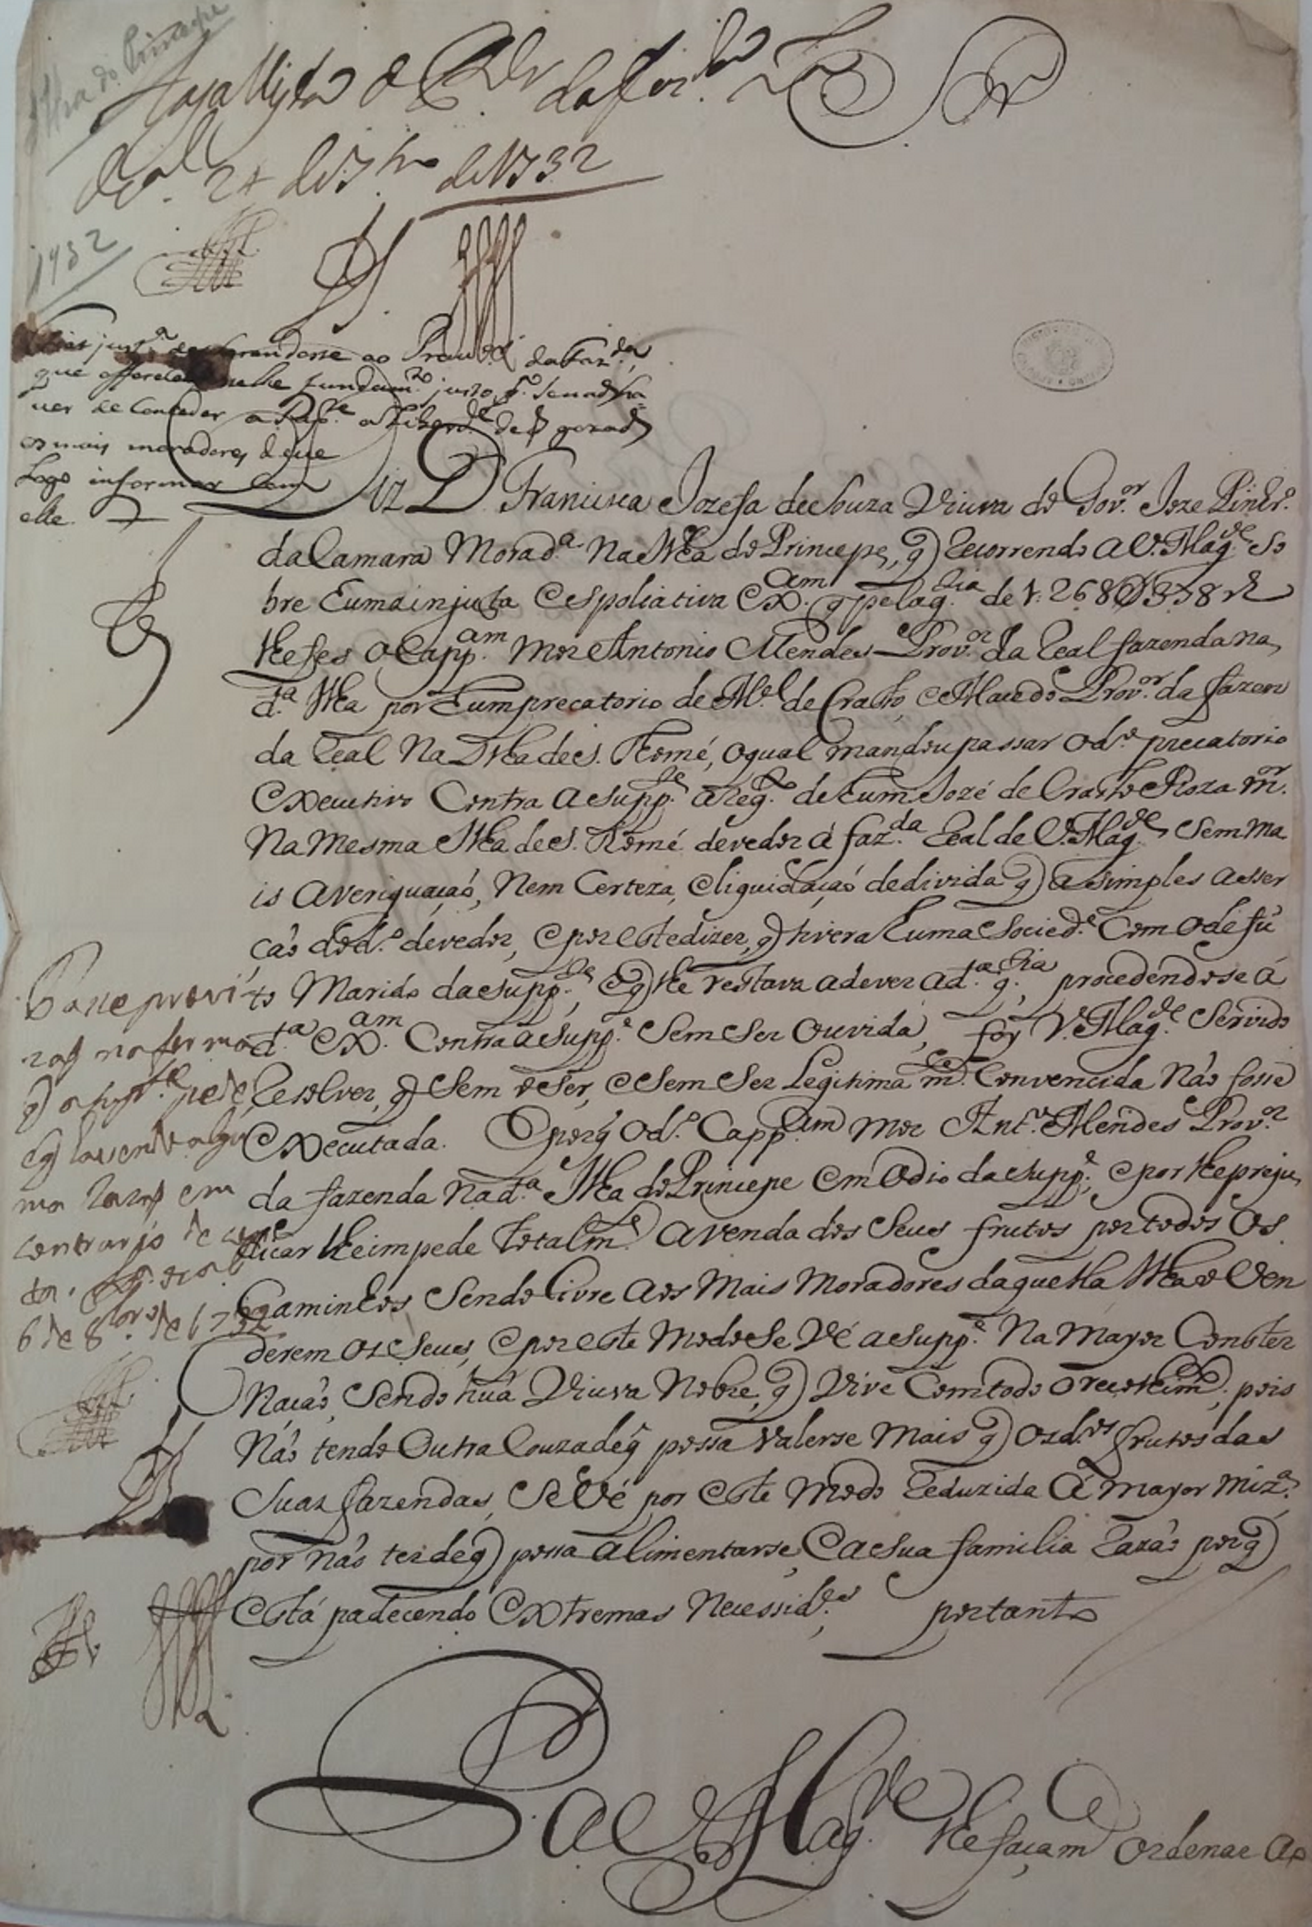
\includegraphics[scale=0.27]{original.pdf}
\caption{Petition of Francisca Josefa de Sousa to King John V (1732). Source: Original documents from São Tomé and Príncipe Islands. Arquivo Histórico Ultramarino, CU\_070, cx. 6, doc. 650.}
\label{fig:original}
\end{figure*}

\begin{figure*}
	\centering
	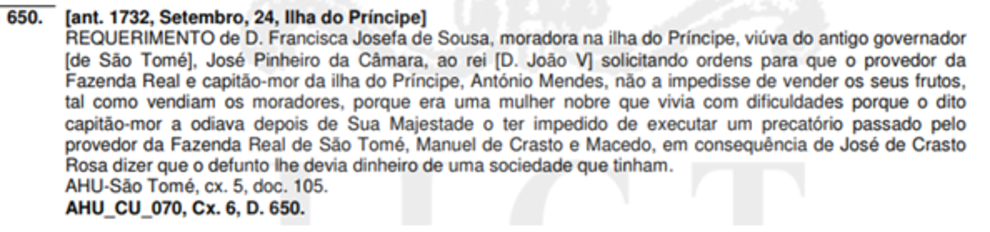
\includegraphics[scale=0.75]{catalog.pdf}
	\caption{The catalogue entry corresponding to the petition of Francisca Josefa de Sousa to King John V shown in Figure \ref{fig:original}.}
	\label{fig:catalog}
\end{figure*}

The administrative correspondence we analyze reflects complex social and political processes such as the early-modern colonial dynamic, global interactions, construction of formal empire, and the evolution of the Portuguese multi-continental monarchy. We believe the biggest advantage of this particular data source is the fact that, contrary to what Ahnert and Ahnert \cite{ahnert_protestant_2015} expressed about archival data, it is not so much subject to the bias of a private letter collection. Yet, it is still subject to the vicissitudes of time as it is impossible to determine how many documents could have been destroyed during the massive fire devastated Lisbon in 1755 as a consequence of an earthquake. It is also difficult to  estimate how many documents could have remained in individual colonies, hence did not make their way to the Archive. These limitations together make the described data alone not ideal to address phenomena occurring beyond the official boundaries of the empire, known as “shadow empire” \cite{hespanha_filhos_2019} or “beyond empires” \cite{antunes_beyond_2016}. 

At this stage of creating our dataset, it is also not possible to carry out linguistics-based coding approach \cite{franzosi_narrative_1998} nor to evaluate what type of relationship the sender maintained with the recipient \cite{kenna_maths_2015}.  Firstly, it is not possible to manually annotate tens of thousands of documents. Secondly, the short description of the letter does not contain all the expressions that are included in the original text. Our dataset has been created mainly to identify all key social actors, their occupation, and the institutions they represent. It is possible, however, that in the subsequent stages, we could use the linguistic approach and semantic grammar to group the correspondence according to the subject matter, as the colonial representatives used to discuss each problem in separate letters. Thus, we could use this method to compare the amount of correspondence concerning the politics, economy, coast defence, piracy, tax issues, etc. Then, we could also use topic modeling to classify the documents according to the topic, by labeling key-words and manually annotating the selected letters \cite{wittek_supporting_2011}.

\section{Historical network research}

The use of network analysis for historical research is becoming increasingly popular for different historical periods. The pioneering research of John Padgett and Christopher K. Ansell \cite{padgett_robust_1993} showed how analysis of networks helped in understanding the state-building of Florence in the 15th century and how the political power of the Medici family emerged. However, the diversity of documents from different historical periods means that there is no one common approach to this type of analysis \cite{mclean_circulation_2014}. Even more relevant for us is the research on historical correspondence documents originating mainly from the early modern period. We believe that the early-modern correspondence networks can reflect a long-distance construction of social ties. Letters represented social connections and were the means to negotiate complex personal ties with different protagonists. Letters, indeed, revealed how individuals shaped networks, constructed their social environment and connected with others. Besides, they enable to link "micro-level practices to macro-level institutional developments" to better understand the administrative changes and emergence of the state \cite{mclean_art_2007}. 

Historical network research based on the correspondence such as protestant lett0per networks \cite{ahnert_protestant_2015} and early modern nuns’ letters \cite{mcshane_visualising_2018} reveal the main protagonists by focusing on the role of recipients and senders ranked by in-degree and out-degree, while in the early modern patronage letters it possible to extract different rhetorical patterns observed in communication exchanged between different social agents \cite{mclean_art_2007}. Research projects as ``Mapping the Republic of Letters''\footnote{``Mapping the Republic of Letters'' is available here: \url{http://republicofletters.stanford.edu/}.} \cite{edelstein_historical_2017}, ``Cultures of Knowledge: Networking the Republic of Letters, 1550-1750''\footnote{``Cultures of Knowledge: Networking the Republic of Letters 1550-1750'' is available here: \url{http://www.culturesofknowledge.org/}.}, ``Circulation of Knowledge and Learned Practices in the 17th-century Dutch Republic''\footnote{``Circulation of Knowledge and Learned Practices in the 17th-century Dutch Republic'' is available here:  \url{http://ckcc.huygens.knaw.nl/}.} \cite{roorda_letters_2010,van_den_heuvel_mapping_2015,van_den_heuvel_circles_2016} and ``The Reception and Circulation of Early Modern Women's Writing, 1550-1700''\footnote{``The Reception and Circulation of Early Modern Women's Writing, 1550-1700'' is available here: \url{http://recirc.nuigalway.ie/}.} \cite{booth_only_2017,coolahan_material_2017} offer both, a deeper understanding of personal relationships among European intellectuals, to better explain how some ideas spread within an intellectual community and provide an insight into mixed-methods approaches while applying the social network analysis in the historiographic studies. 

In the successive stages of our research, we will follow the mix-method approach \cite{martinez_combining_2003,dominguez_mixed_2014}, that consists first on determining critical questions based on a quantitative analysis that we follow up with the qualitative one. Combining both methods can result in a better-integrated study that reduces limitations of each approach \cite{crossley_social_2010}. Besides, it is “mutually informative” and provides a “cross-referencing tool to test the reliability of network” \cite{edwards_mixed-method_2010}, and identifies “inconsistencies and contradictions” between both methods \cite{padgett_economic_2011}. 

While it is not the purpose of this article to deepen the qualitative methods concerning the colonial empire-building. Nonetheless, it might be important to briefly explain the next stages in our research. Considering the above research on the early modern sources and mixed-methods approaches, we also aim to combine the traditional historiography on the Portuguese empire with methods of social network analysis to study archival records stored in the Portuguese Overseas Archives.  It is worth highlighting that understanding the colonial Portuguese world through networks in the theoretical perspective of trans-imperial and cross-cultural connections \cite{ribeiro_da_silva_trans-imperial_2018} or political correspondence \cite{fragoso_um_2017} has been the subject of research in recent years at the Luzo-Brazilian Academy. However, it has not been approached on such a large scale yet.

\section{Defining main characteristics of the type and the content of the Portuguese letters}

Similarly to the research papers examining the correspondence network \cite{mcshane_visualising_2018,ahnert_protestant_2015}, we consider the following elements of correspondence essential to our database: date, type of document, place of sending the document, sender, recipient, content of the document, and any third parties involved in text. These elements are unfortunately not readily available as metadata and thus need to be extracted from the content. Each document contains a specific date in the form of a day, month and year. Sometimes these dates were given as approximate or determined by the Portuguese archivists, hence containing only the year. Figure \ref{fig:records_year} shows the evolution of the number of documents per year, in the period of our analysis (1642-1822). The increase in correspondence in the Atlantic space during the reign of John V reflects the changing policies of the Lisbon metropolis, which previously focused on the Portuguese State in India. For the period of the monarchs Joseph I and Maria I, however, the consequences of the 1755 earthquake in Lisbon might have had a strong impact on decreasing the circulation of correspondence between the destroyed capital of the empire and its colonies.

\begin{figure*}
	\centering
	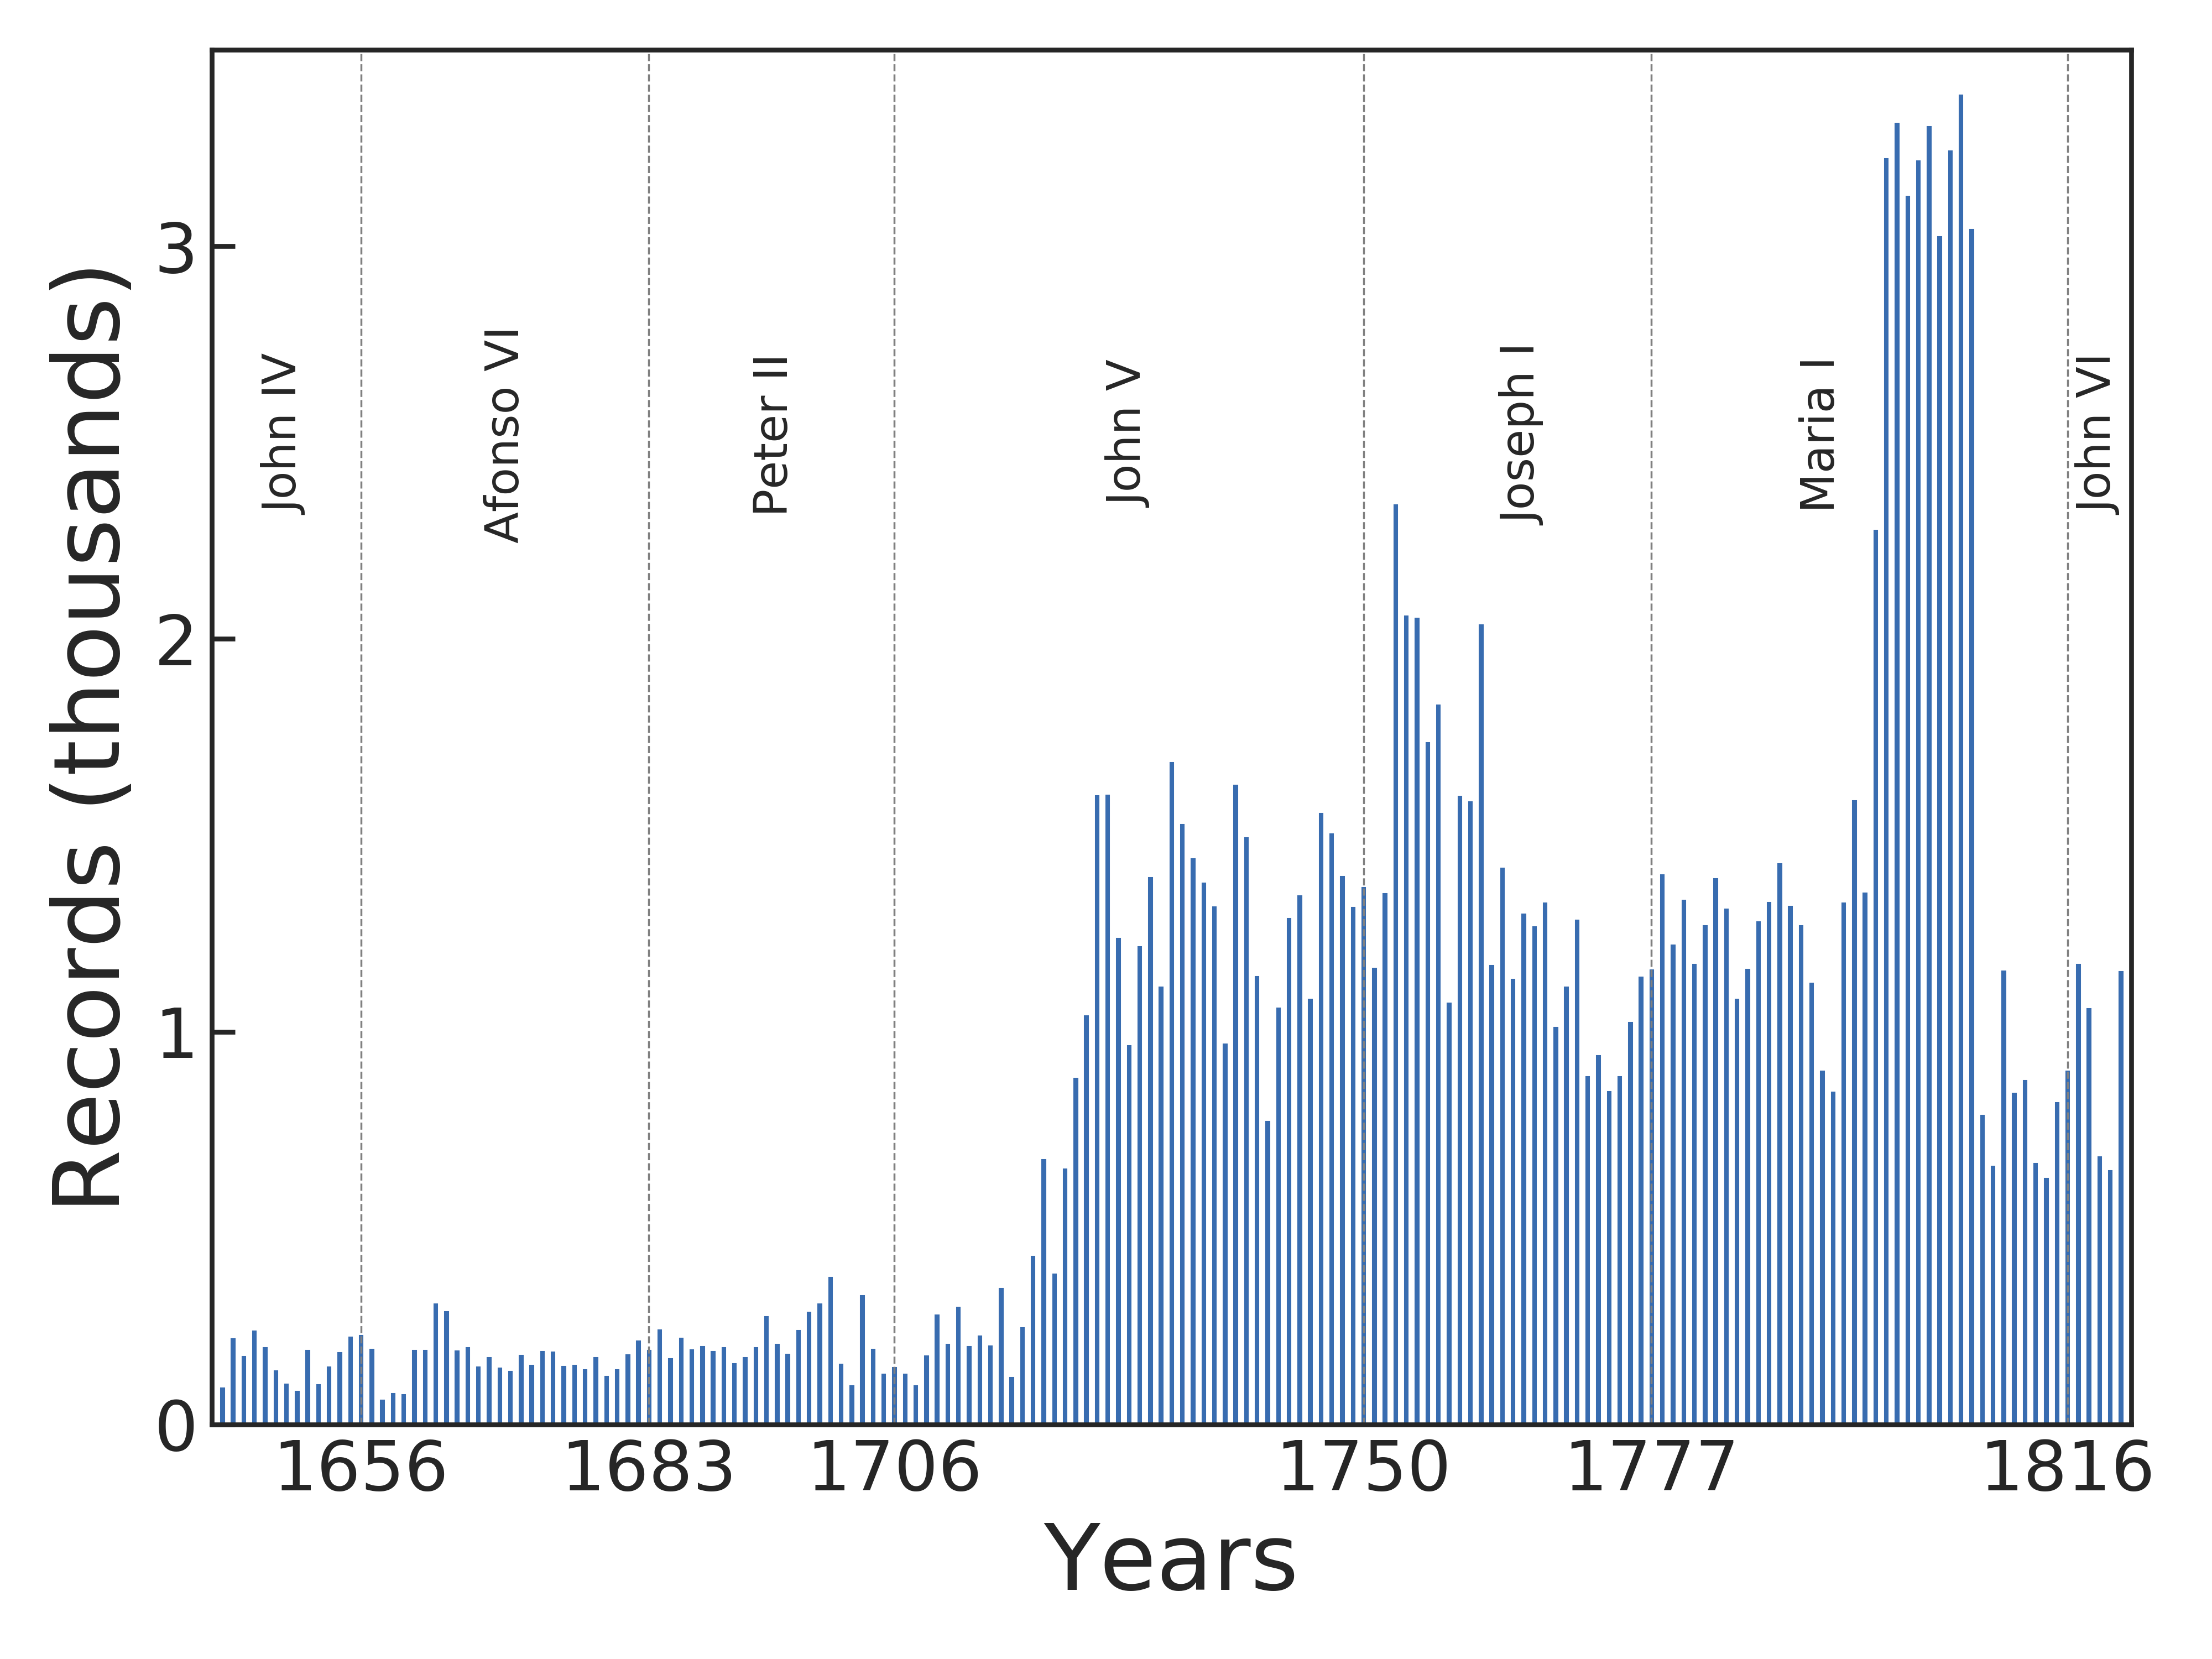
\includegraphics[scale=0.40]{records_per_year_1642-1822.png}
	\caption{Evolution of the number of records in the period chosen for our analysis (1642-1822). Gray dotted lines correspond to years in the x-axis, when there was a transition of monarchs.}
	\label{fig:records_year}
\end{figure*}

The archivists also classified the documents into over five hundred categories according to their type. The most frequent types are: Requerimento (Petition), Ofício (Circular), Carta (Letter), Consulta (Enquiry), and Aviso (Notice), as shown in Figure \ref{fig:doc_types}. It seems that the classification is not always standardized. For example, we noticed that some seventeenth century documents labelled as Carta (Letter) reveal a similar writing pattern and content as in the eighteenth century documents labelled as Requerimento (Petition). Some documents are not really a correspondence per se. In particular, they do not have a relational character with a defined sender and recipient. These documents usually refer to an administrative decision, such as Bilhete (Ticket), Passaporte (Passport) or contain only maps or tables.

\begin{figure*}
	\centering
	\subfigure{\label{fig:freq} 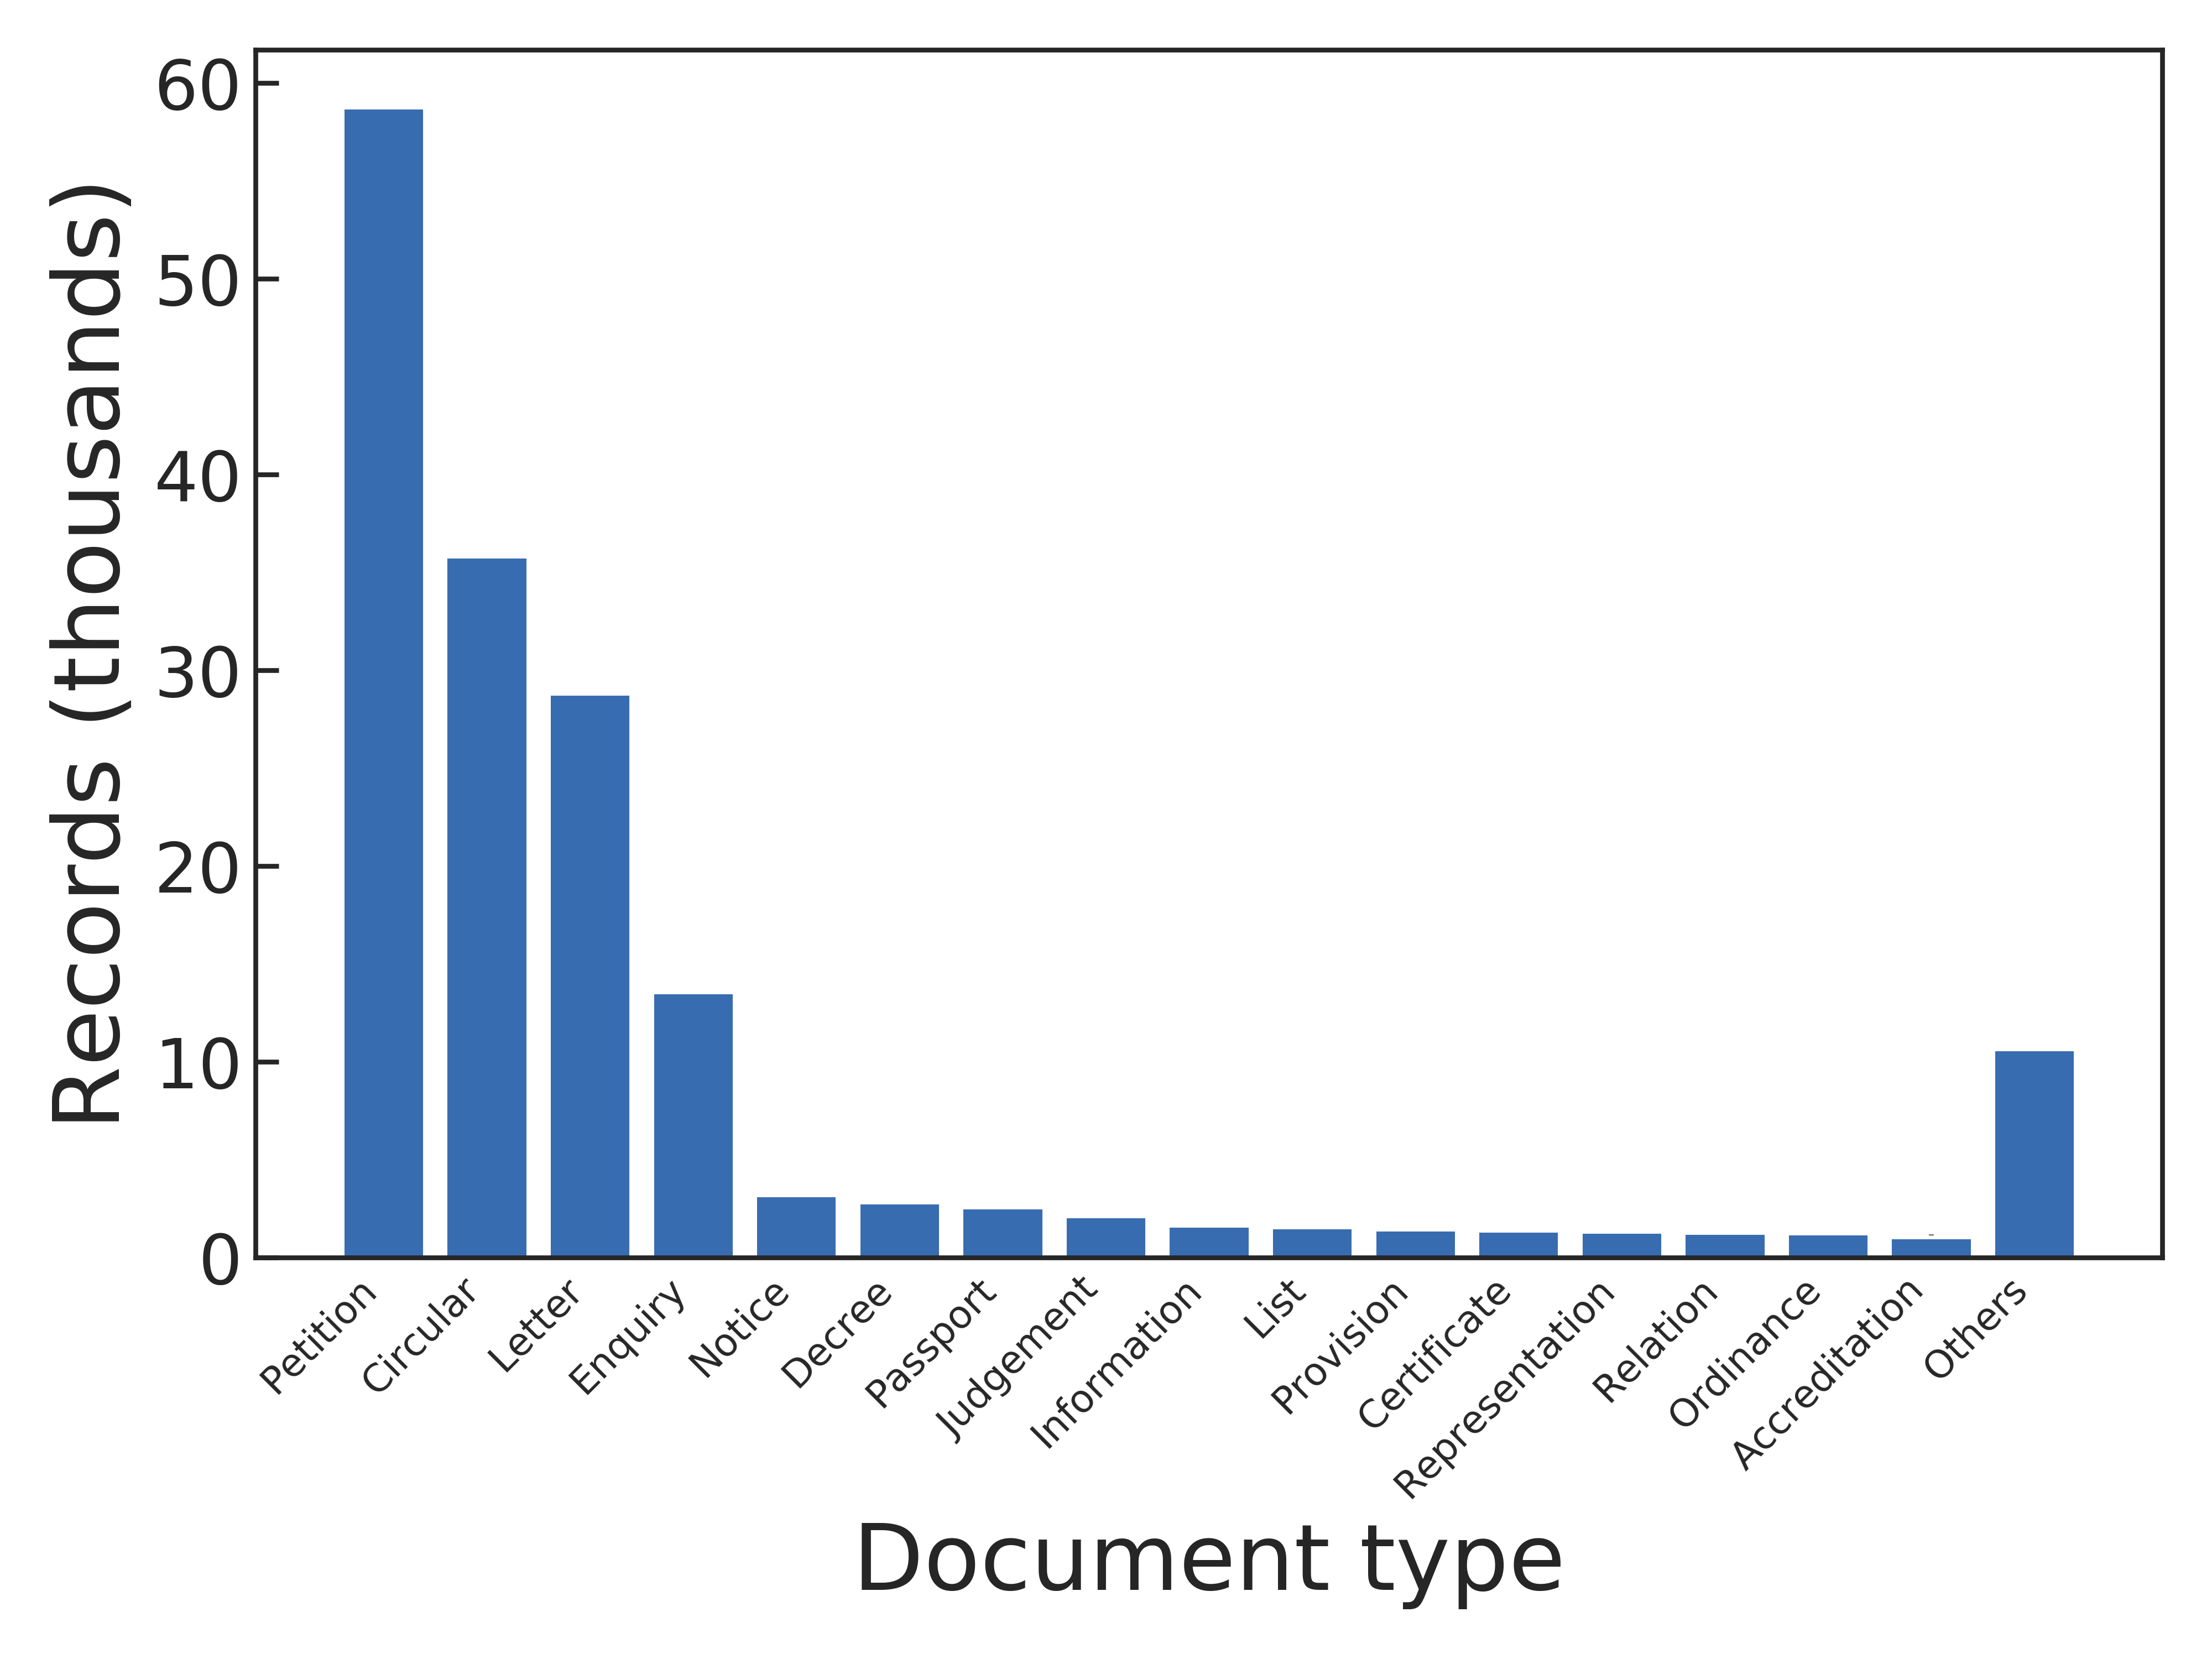
\includegraphics[scale=0.35]{doc_type_frequency_1000.png}}
	\subfigure{\label{fig:evol} 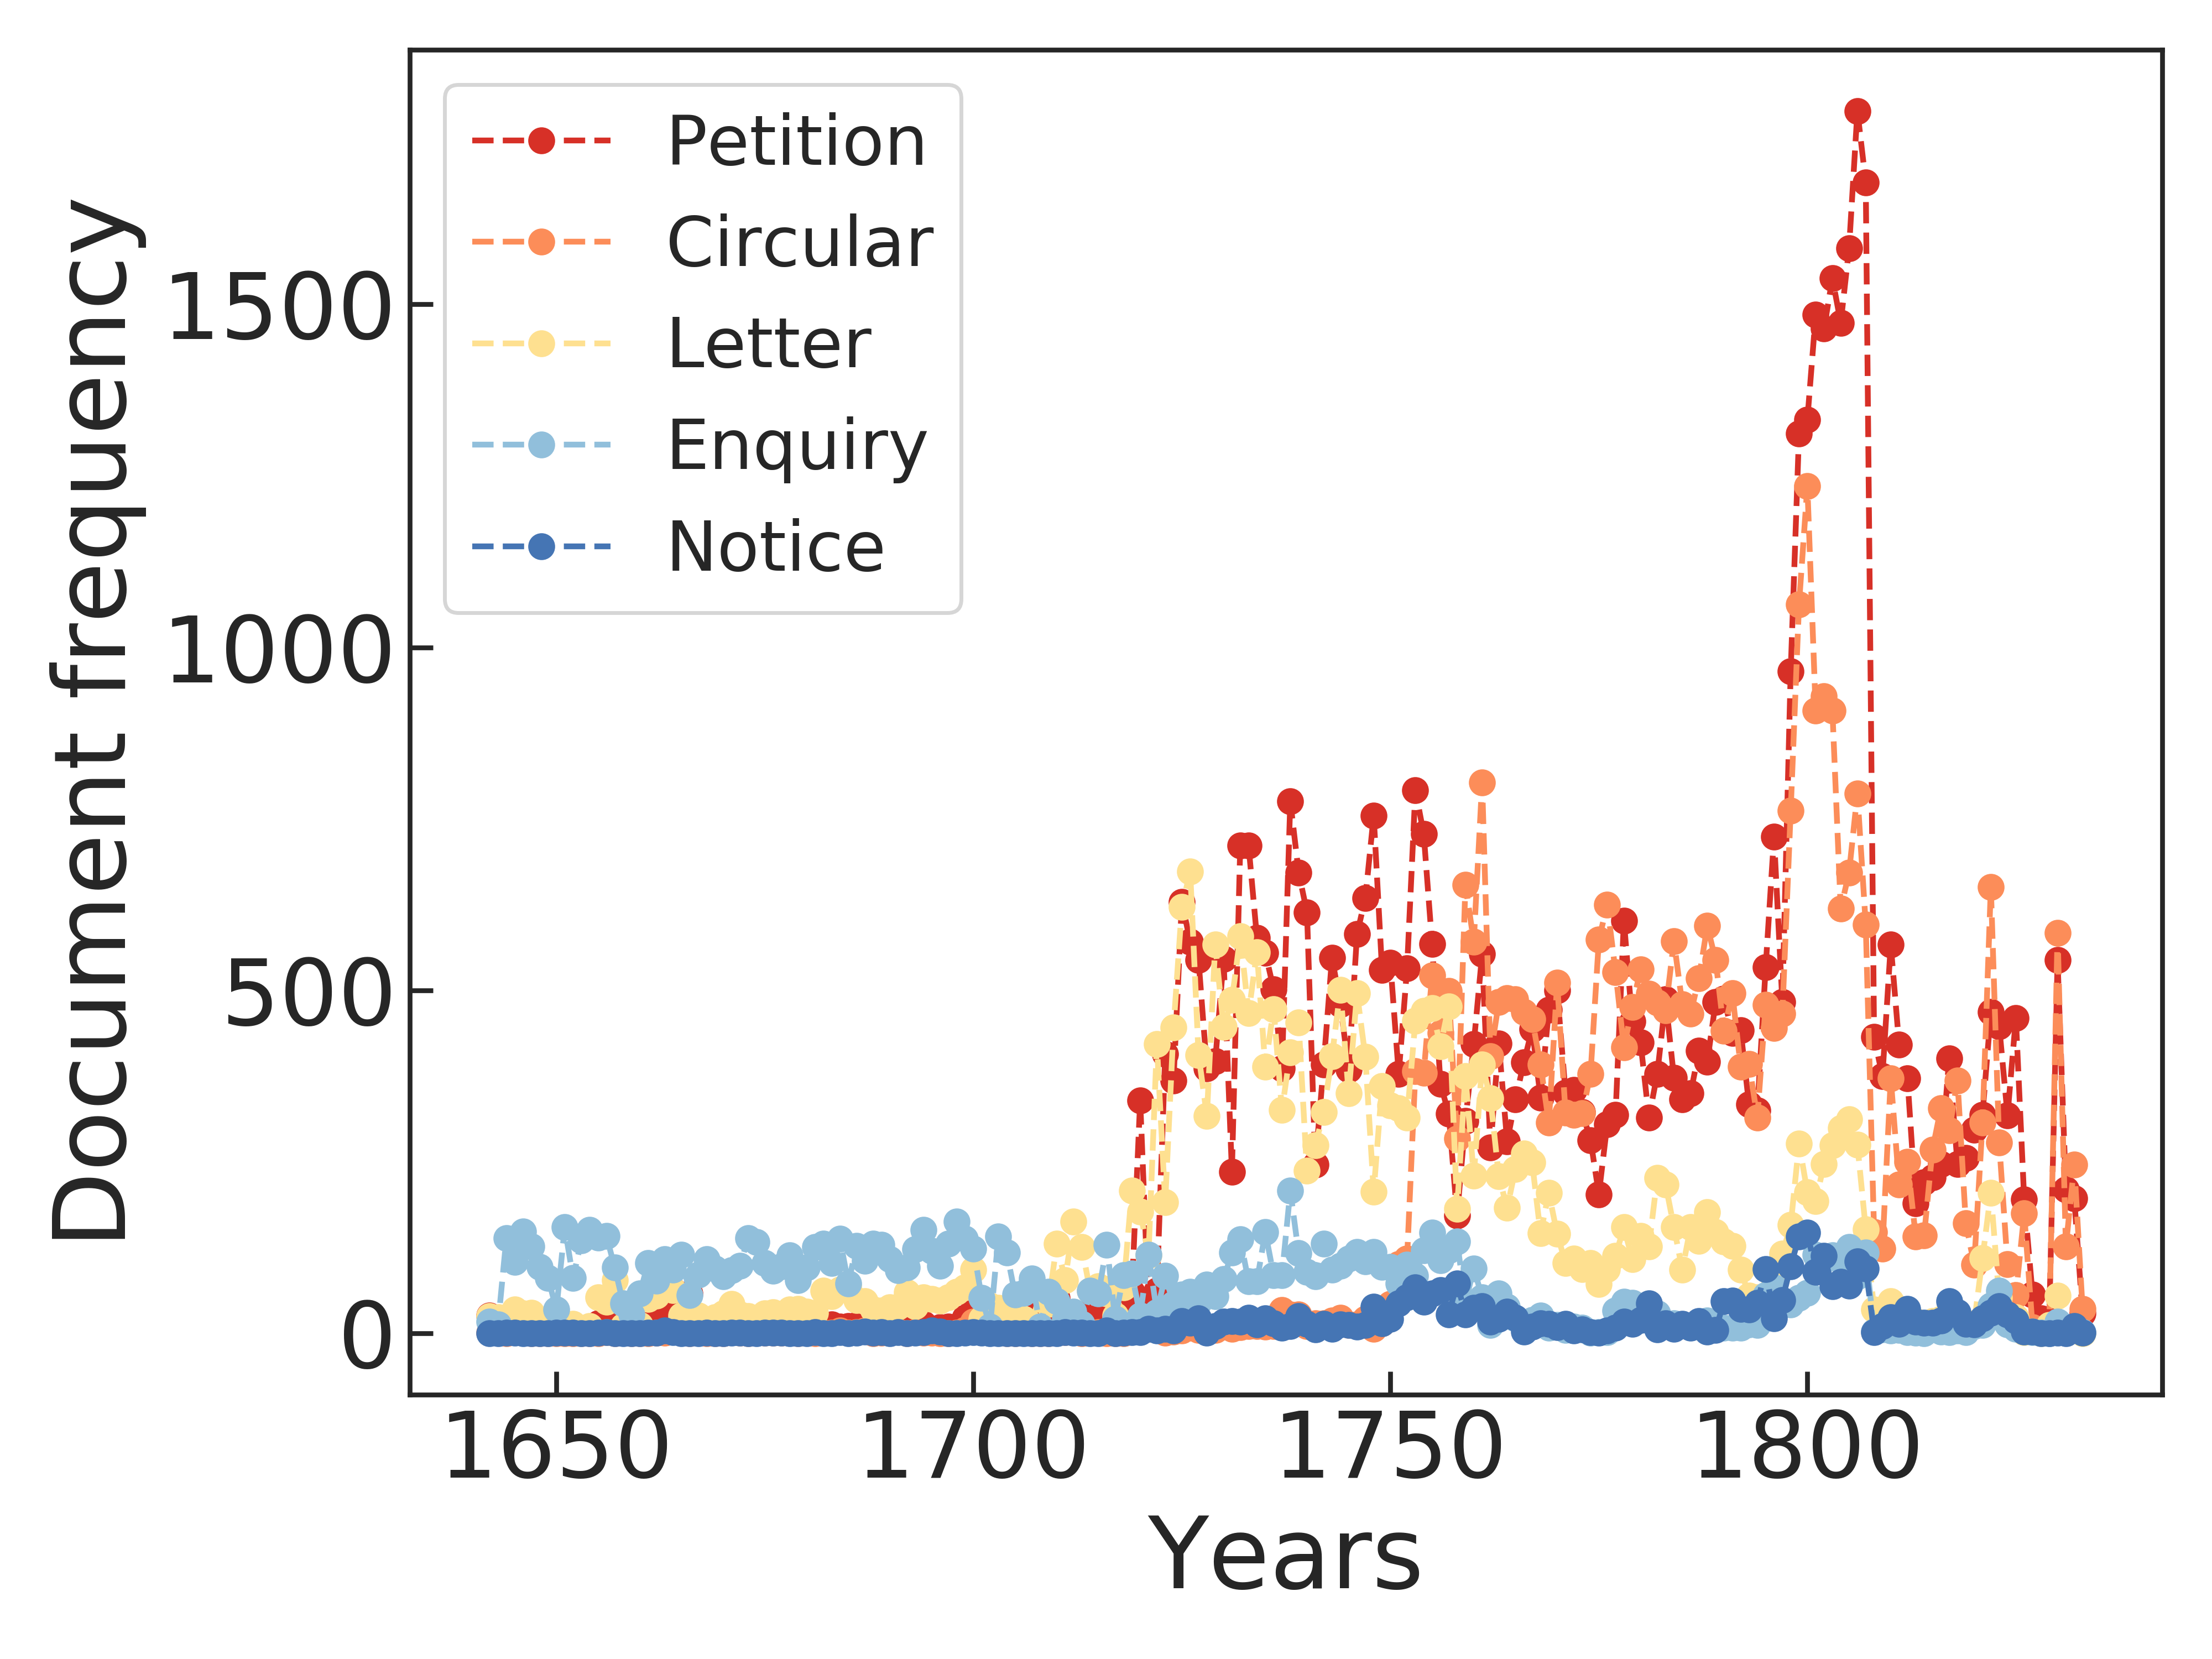
\includegraphics[scale=0.35]{top5_types_evolution.png}}
	\caption{Left: number of records per type. Right: evolution of the number of documents per type of the five most frequent document types.}
	\label{fig:doc_types}
\end{figure*}

Determining the place of sending the document was facilitated by the meticulous work by the members of the Overseas Council since the seventeenth century, who segregated them under geographic criteria, always keeping chronological order \cite{arquivo_historico_colonial_boletim_1950}. In the case of the Brazilian colony, it should be noted that it was not perceived as one territorially integrated area, but initially as a “hereditary captaincies” and then states. The great challenge, however, was to identify the place from where the document was sent, taking into account the fact that some places were given the original names that are no longer used, while some other places do not exist anymore, like a sugar cane plantation or a village. Generally speaking, the letters were usually sent from very different cities in the case of Brazil, and from major strategic cities, ports or fortalezas (fortresses) in the case of Africa. Figure \ref{fig:records_state} presents the number of records in our corpus, from every identified place of origin.

\begin{figure*}
	\centering
	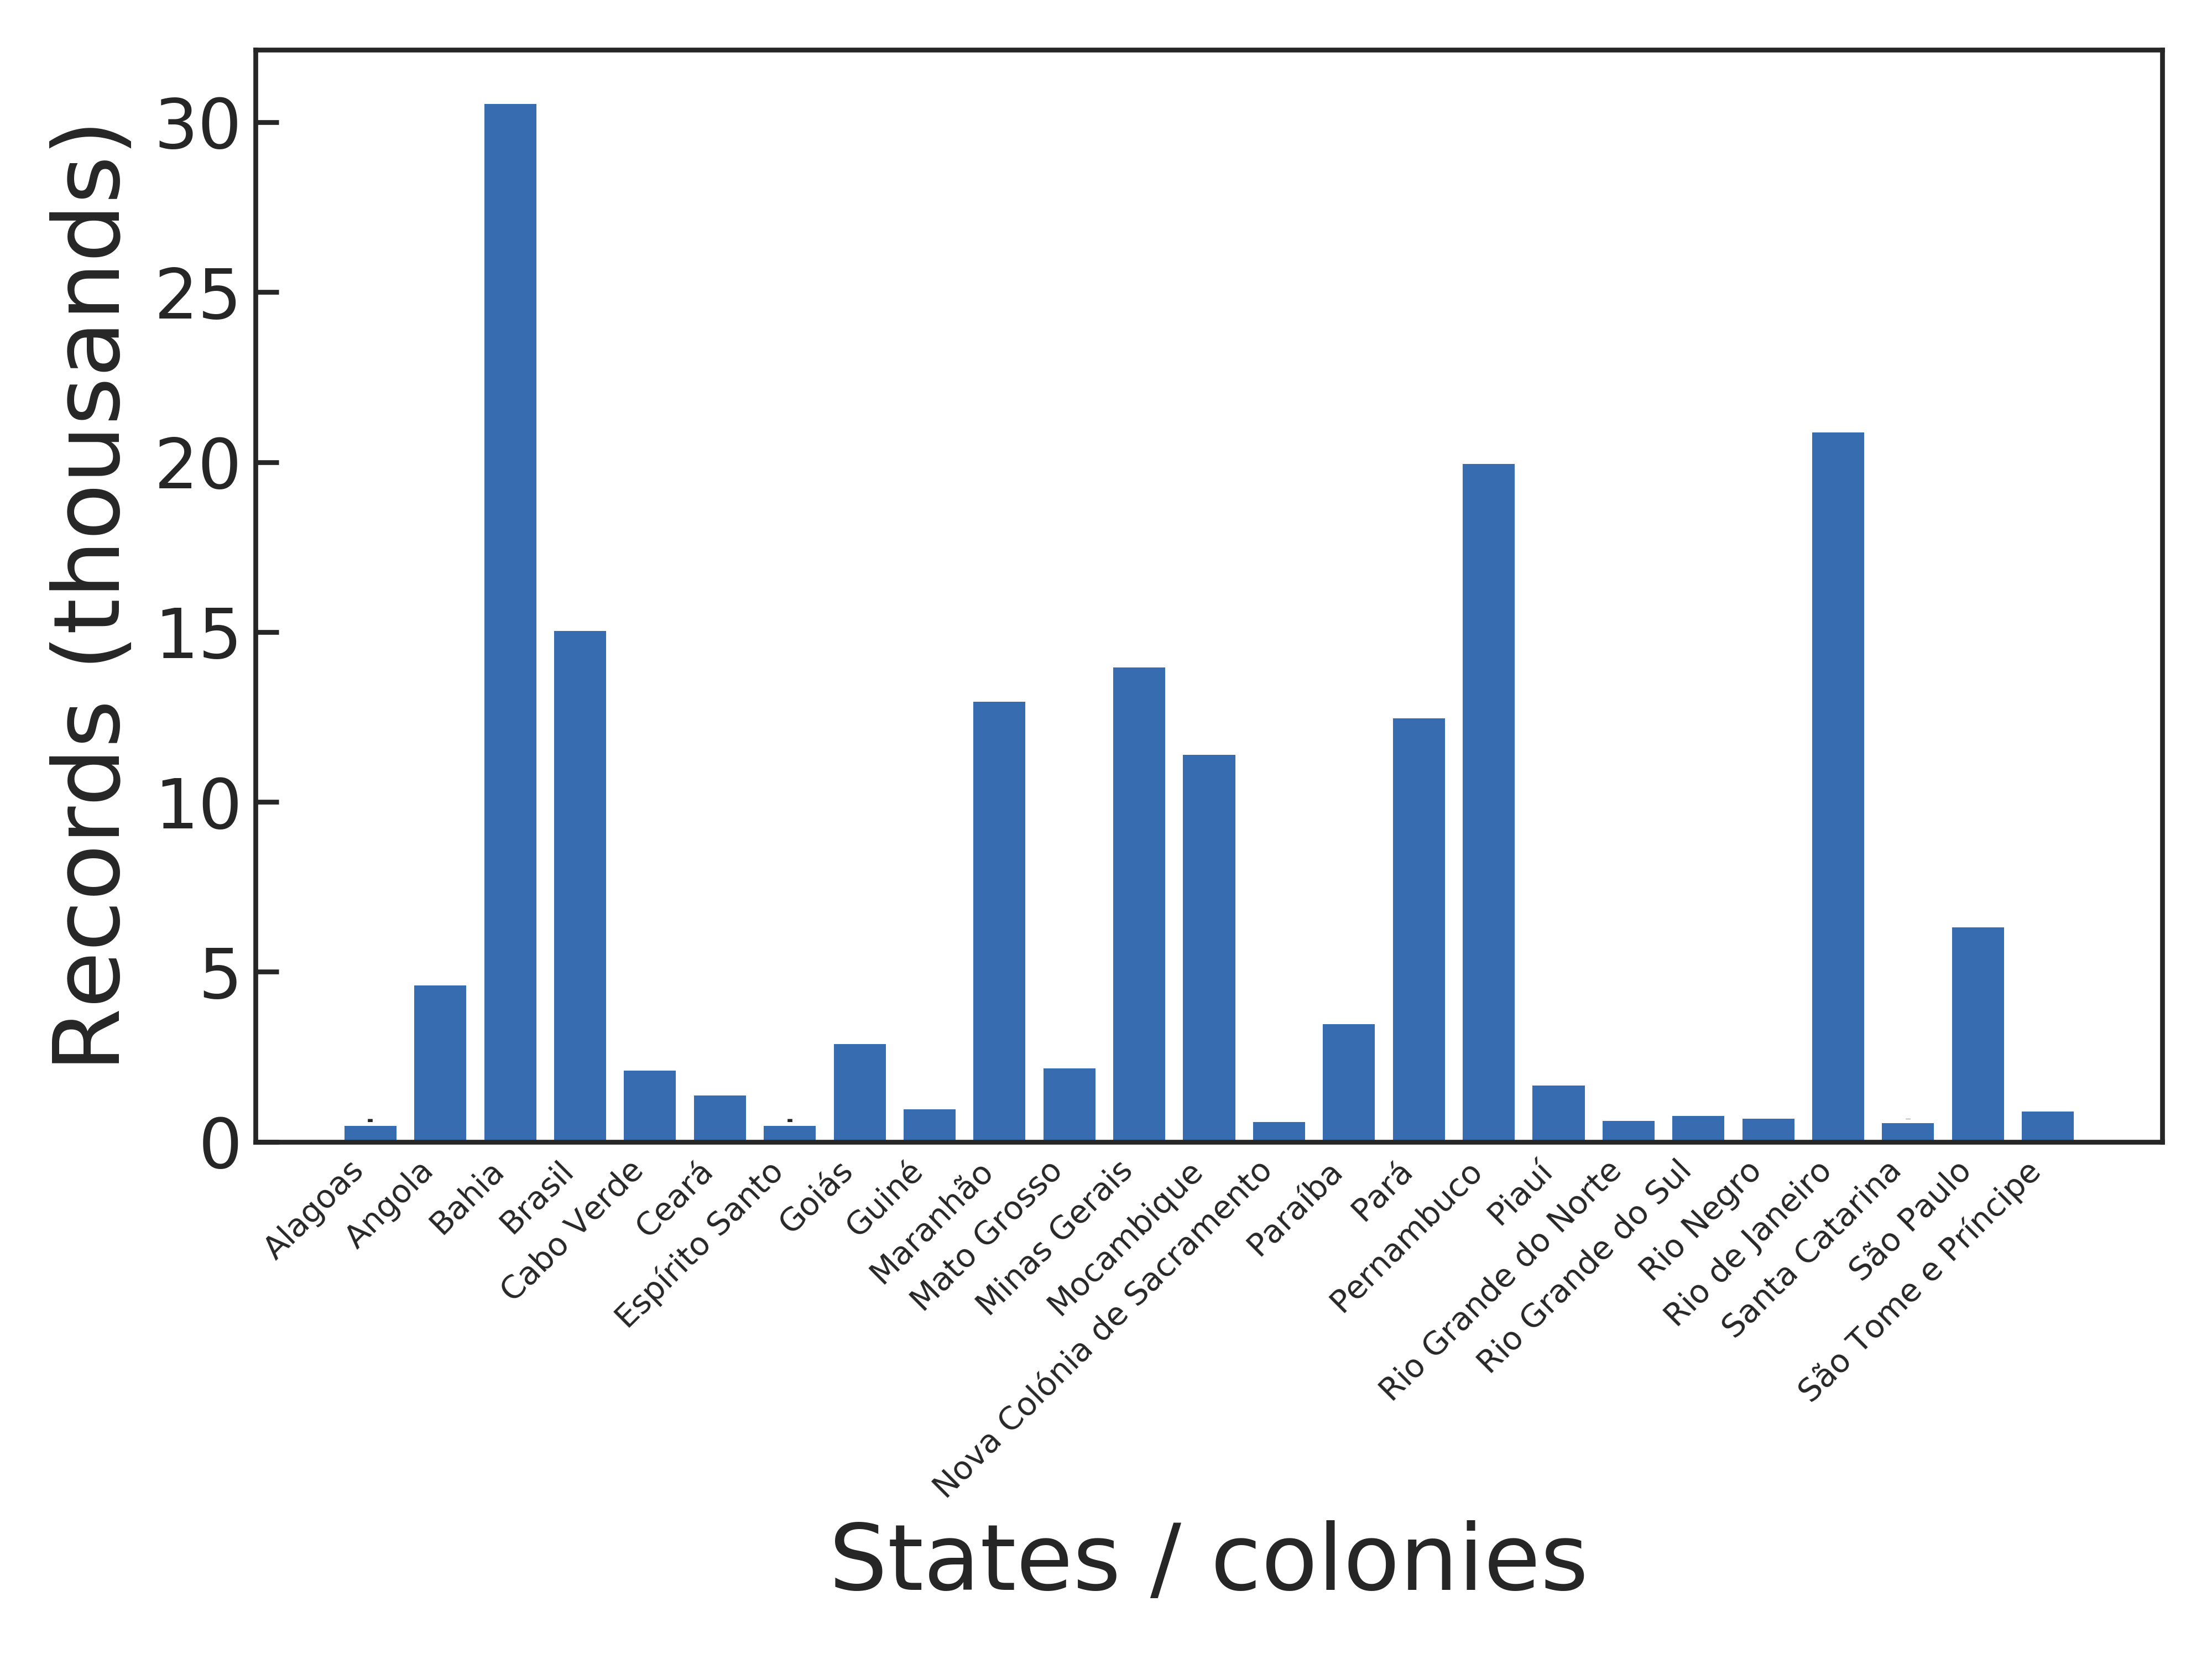
\includegraphics[scale=0.40]{records_per_state.png}
	\caption{Number of records for every place of origin (localization of the sender) identified.}
	\label{fig:records_state}
\end{figure*}

The senders of the letters are both secular (e.g. municipal chambers) or religious institutions (e.g. brotherhoods), as well as colonial officials (as governors and viceroy, for instance), clergy (bishops, priests), military personnel (soldiers, captains), or the individuals,  both women and men, regardless of their social status (indigenous, slaves), or colour (“black”, “mulatto”, etc.). The most frequent recipient of all this correspondence was the Lisbon administration. The letters were most often addressed to the Portuguese monarchs, the Overseas Council and secretaries of state, all residing in Lisbon. It is worth noting that there was also internal communication, that is some letters were sent to the governors of a colony or a state, and this type of communication was very characteristic for Mozambique.

There is a substantial diversity in topics that were the subject of letters sent to and from Portugal. The ones sent from the overseas possessions often contain information on the social, administrative, political, religious, and economic character. The inhabitants of the Atlantic colonies informed their recipients about the exotic products, culture, people, plants and animals. They shared their memories as settlers, informed about the socio-political situation, including indigenous, fortune hunters Bandeirantes, intermediaries Pombeiros, pirates, as well as about the economic situation referring to different plantations. The colonial settlers often petitioned, hoping for a favorable solution to their problems, additionally to asking the king to provide them with self-defense weapons, and complaining about the inefficiency of the system. In turn, the Lisbon administration used to inform them in the form of instructions named Carta Régia (Royal Charter), Regimento (Regulation), Lei (Law), Provisões (Provisions), Consultas (Consultation), and Instruções (Instructions) that addressed the politics, economy or the secular and religious power structures. The colonial residents were also instructed on how to wage war against the natives, or how to plant sugar cane, build fortresses, maintain the peace, buy slaves, run transatlantic trade or extract precious stones from the mines \cite{boschi_o_2011}.

\section{Natural Language Processing and text analysis}

In this section, we discuss the steps of the methodology we used in the whole process of turning the raw data into network data. Figure \ref{fig:methods} shows a diagram with a summary of the steps of our methodology. In a nutshell, these steps are:
\begin{enumerate}
	\item Creation a random sample from the 169,221 records in plain text ready for annotation.
	\item Annotation of records in the sample, with the labels (categories) of our interest.
	\item Named Entity Recognition (NER) model training with the annotated records.
	\item Extraction of metadata from all records and recognition of text pattern, both with regular expressions.
	\item NER parsing to identify the entities present in all records.
	\item Creating of network data with an analysis of duplicate entities and corrections of typos.
	\item Network analysis and visualization.
\end{enumerate}

We will discuss these steps in more detail in the next two subsections and Section 6.

\begin{figure*}
	\centering
	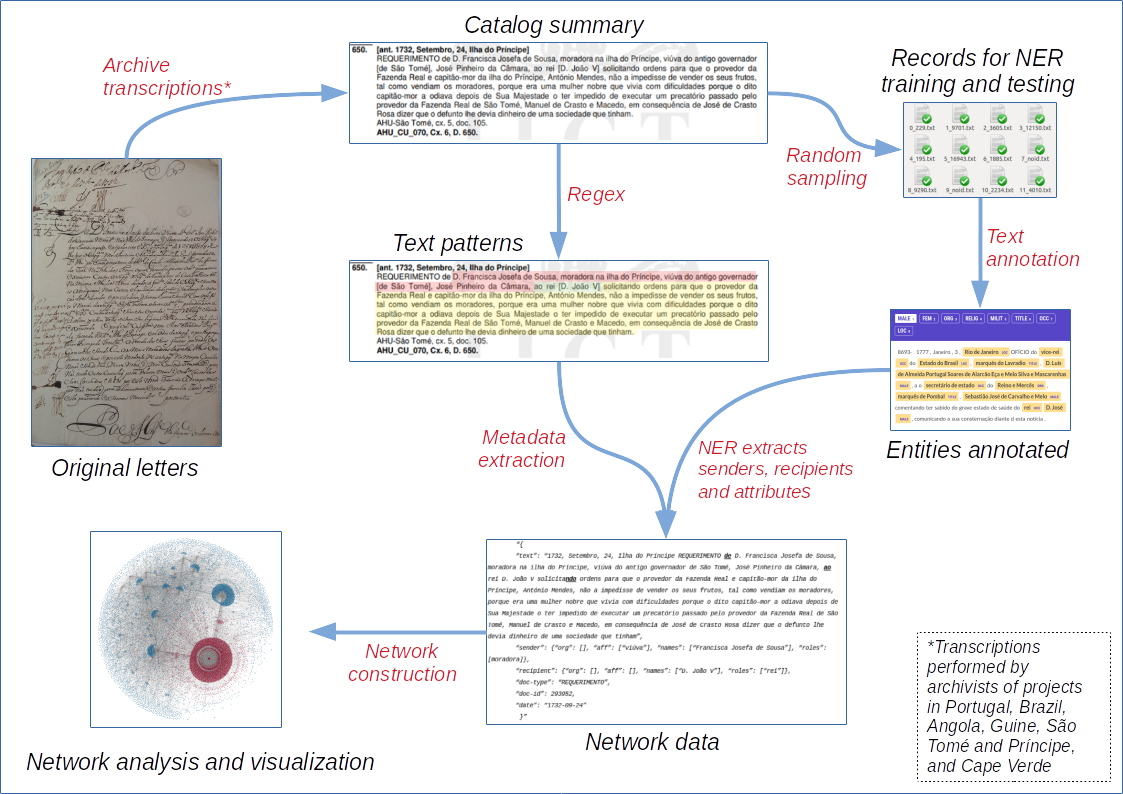
\includegraphics[scale=0.40]{methods_diagramv2.png}
	\caption{Schematic of the methodology to turn archive data into network data.}
	\label{fig:methods}
\end{figure*}

\subsection{Identifying the entities mentioned in the letters}

We have seen in the previous section that the correspondence records of the Portuguese Overseas Archive collection, in the Avulsos type, have several distinct forms as well as a heterogeneous set of actors (senders and recipients). We identified these actors, and most of their attributes, using the Named-entity Recognition (NER) tool of the Natural Language Processing (NLP) library for Python called spaCy\footnote{Information on SpaCy is available on \url{https://spacy.io/}.}. The function of the NER tool is to parse plain texts (the records were originally in PDF format, then converted to plain text) to locate and identify the entities mentioned in such texts. Then, the tool classifies these entities into previously defined categories, e.g. people, institutions, locations, products, events, and so on.

Our first big challenge when using natural language processing techniques in this study was the fact that our texts are in Portuguese. Even though there exist libraries to perform NER in the Portuguese language, these libraries still are relatively small, without a large diversity of texts. As a consequence, although the reported accuracy for Portuguese reaches 89\%, for the spaCy v2.2 NLP library\footnote{Information on SpaCy models is available on \url{https://spacy.io/models/pt}.}, in practice the accuracy can be much lower, especially for documents from the 17th until the beginning of the 19th century. Terms of such periods makes it more difficult for the NER analysis, as many names and locations are not frequently used anymore. Many of these names do not appear in the current text libraries used as a reference for the NER model.

Our second big challenge was that the variety of the correspondence records, their complexity, and the time-span made it difficult for the right categorization of the entities. The standard Portuguese NER model in SpaCy has only four entity categories: PER (for persons), LOC (for locations), ORG (for institutions in general), and MISC (miscellaneous - for any other entity), which is not enough for our purposes. We wanted to enrich our network data with information such as gender, occupation, and nobility title, if any, of actors.

To overcome the issues mentioned above, we decided to train a new Portuguese model from scratch. For that, first, we created a random sample of 4,230 registers --- corresponding to 2.5\% of the total. Secondly, we manually annotated the entities and their type, for every entity found in these records. To that end, we used the software Prodigy\footnote{Information on Prodigy is available on \url{https://prodi.gy/}.} which helps in the task of annotating texts. Figure \ref{fig:prodigy} shows an example document with manually marked text fragments referring to entities of our interest labeled with the proper categories. 

\begin{figure*}
	\centering
	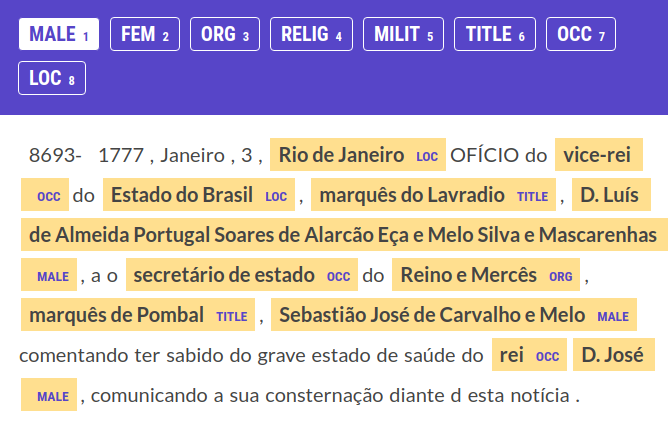
\includegraphics[scale=0.40]{prodigy.png}
	\caption{Example of annotating record with Prodigy. In this case we have LOC - Rio de Janeiro, and Brasil; OCC - vice-king, secretary of state, and king; TITLE - marquis of Lavradio, and marquis of Pombal; MALE - D. Luís de Almeida Portugal Soares de Alarcão Eça e Melo Silva Mascarenhas, Sebastião José de Carvalho e Melo, and D. José.}
	\label{fig:prodigy}
\end{figure*}

We split PER into MALE and FEM. For MALE we decided to annotate all the complete male names, for instance Antônio Teixeira de Mendonça. For practical reasons, we decided that the abbreviation of the noble Portuguese title Dom should be annotate together with the name, as it was in the case of D. João d'Ávila. We performed analogically with FEM, we annotated such forms as Ana Maria Nogueira, D. Joana or Dona Maria Braga. To track nobility titles, we created a separate category named TITLE, including for instance Marquis of Lavradio and Count of Oeiras. For the categories of the administrative and political structure, due to such a diverse character of colonial entities in terms of linguistics, we decided to divide them into three categories. The first is ORG, which contains all civil and secular establishments of a purely administrative-political character, such as Conselho Ultramarino (Overseas Council) or Casa de Suplicação (Tribunal). We adopted the same practice in the category RELIG and MILIT, for religious and military institutions, respectively. The category OCC includes all words relating to professional occupation, for instance governor (governor), soldado (soldier) or juiz (judge).  Finally,  for the category LOC we decided to annotate not only cities, states and countries, but also several locations like villages such as Vila de Massangano, rivers as Rio São Francisco, and military fortresses in Africa known as presídios, as Presídio de Pedras Negras. This way, we are able to identify more detailed information about the localization of the events described in the records. We didn’t use the MISC category.

With all the over four thousand records annotated, we trained our NER model. We used 80\% of all annotated records to actually train the model and the other 20\% to test it. As a result of the test, we reached 93,1\% of accuracy in recognizing the eight categories of entities.

\subsection{Finding patterns}

After the identification and classification of the entities, our next step was to identify who were the sender(s) and the recipient(s) of the letters. For that, we had to distinguish possible patterns in the structure of the text of each correspondence record that would characterise the activity of the entity as a sender or a recipient. In general, the records (the petitions in particular) present the following segments: senders and their attributes (if existent), recipients also with their attributes (again, if existent), and a summary of the main content of the correspondence.

That way, by using regular expressions techniques, we could divide the text of each letter into three segments, with the following reasoning. First, we located the presence of Portuguese prepositions such as de, do, da, dos, das (in English: from and from the) and set these words as the start of the text segment with information regarding the sender of the letter. Second, we located other prepositions as a, à, ao, às, aos, para (in English: to and to the), as the end of the sender segment and the start of the recipient segment. Finally, we located verbs in the gerund form (in Portuguese verbs ending with ndo, in English: ing), indicating some activity as, for instance, asking, claiming, protesting, stating, declaring, and so on. The verbs in the gerund form are set as the end of the text segment related to the recipient, and the start of the segment with the content summary.

Below is an example of a processed record that we created, stored in JSON format, after the named-entity recognition and the identification of senders and recipients, as well as their attributes. This is the petition - the original and the record are shown in Figures \ref{fig:original} and \ref{fig:catalog}, respectively - sent by Francisca Josefa de Sousa, addressed to King John V. The characters marked in bold and underlined are the words used to identify the three segments of text as stated above. In “aff” we store the actors’ affiliation to institutions, be it ORG, MILIT or RELIG.

\begin{quotation}
\noindent
\textit{
``\{ \\
	``text'': ``1732, Setembro, 24, Ilha do Príncipe REQUERIMENTO \textbf{\underline{de}} D. Francisca Josefa de Sousa, moradora na ilha do Príncipe, viúva do antigo governador de São Tomé, José Pinheiro da Câmara, \textbf{\underline{ao}} rei D. João V solicita\textbf{\underline{ndo}} ordens para que o provedor da Fazenda Real e capitão-mor da ilha do Príncipe, António Mendes, não a impedisse de vender os seus frutos, tal como vendiam os moradores, porque era uma mulher nobre que vivia com dificuldades porque o dito capitão-mor a odiava depois de Sua Majestade o ter impedido de executar um precatório passado pelo provedor da Fazenda Real de São Tomé, Manuel de Crasto e Macedo, em consequência de José de Crasto Rosa dizer que o defunto lhe devia dinheiro de uma sociedade que tinham'', \\
	``sender'': {``aff'': [], ``title'': [], ``names'': [``D. Francisca Josefa de Sousa''], \\
	``occ'': []}, \\
	``recipient'': {``aff'': [], ``title'': [], ``names'': [``D. João V''], ``occ'': [``rei'']}, \\
	``doc-type'': ``REQUERIMENTO'', \\
	``doc-id'': 293952, \\
	``date'': ``1732-09-24'' \\
\}''}
\end{quotation}

It is worth to note that one of the biggest challenges was to find the aforementioned patterns in the structure of the correspondence exchanged. Each type of correspondence has its structure, which made it difficult to find a common ground to the analysis of the whole corpus. A direct improvement from this observation, for the next steps in the project, is to create specific algorithms for each type of correspondence. The corpus would have to be heavily fragmented, but this could substantially increase the accuracy of the computer text analysis.

With the above methodology, we extracted vast sets of senders and recipients. The set of recipients is relatively less diverse (as the majority of these letters were addressed to the monarchs and officials) than the set of senders, which is composed of actors ranging from top-ranked government officials to the less favoured individuals such as black slaves and indigenous representatives. While the set of recipients is composed of a little over 9,000 actors, the number of senders amounts to over 40,000 actors.

Due to errors, like typos, found in the registers, we performed a thorough examination of the entities to avoid duplicates, especially of those more relevant to our analysis. That is, we ordered the entities by the frequency with which they appear in the records. Starting from the most frequent ones, we applied an algorithm that compares sequences of characters of a pair of elements \cite{ratcliff_pattern-matching-gestalt_1988}. We used the most frequent version of each entity's name as the reference element and compared every other name in the sets of entities with that. We could fix, for example, instances like ``Fernando José Portugal'' to the corrected version ``Fernando José de Portugal'', and ``Gomes Freire de Andrada'' or ``Gomos Freire de Andrada'' to ``Gomes Freire de Andrade''. Thousands of duplicates were identified and fixed. It is worth noting that we did not apply the algorithm to automatically correct the names of monarchs. Otherwise, names such as ``D. João IV'' could easily be mistaken as ``D. João VI'', for instance.

With the NER model and the segmentation of the texts, we could not only identify senders and recipients of these correspondences but also their attributes. At this stage of the project we are particularly interested in two of them: occupation (OCC) and affiliations (ORG, MILIT, and RELIG), especially the first. Tables \ref{tb:occupations} and \ref{tb:affiliations} show the frequency with which roles and organisations appear, respectively, in the records studied, from 1642 to 1822.

\begin{table}[]
	\vspace{0.2cm}
	%\small
	\centering
	\caption{Frequency with which the roles appear in the documents, for the sender and recipients of the letters. Here we have an indicative of the collective importance of governors (usually also called general captains) in the administrative correspondence of the empire. \label{tb:occupations}}
	\vspace{0.2cm}
	\begin{tabular}{|l|r|l|r|}
	\hline
	\multicolumn{2}{|c|}{Sender}                                      & \multicolumn{2}{c|}{Recipient}                                   \\ \hline
	\multicolumn{1}{|c|}{Occupation} & \multicolumn{1}{c|}{Frequency} & \multicolumn{1}{c|}{Occupation} & \multicolumn{1}{c|}{Frequency} \\ \hline
	Governor                         & 25,867                         & King                            & 42,603                         \\ \hline
	General Captain                  & 10,067                         & Secretary of State              & 27,554                         \\ \hline
	Captain                          & 6,599                          & Prince Regent                   & 17,033                         \\ \hline
	Secretary of Estate              & 5,106                          & Queen                           & 7,814                          \\ \hline
	Provider                         & 4,240                          & Governor                        & 6,813                          \\ \hline
	Vice-Rei                         & 3,664                          & General Captain                 & 3,098                          \\ \hline
	Prosecutor                       & 3,474                          & Captain                         & 1,373                          \\ \hline
	Judge (Desembargador)            & 2,953                          & Master                          & 893                            \\ \hline
	Judge (Ouvidor Geral)            & 2,213                          & Minister                        & 698                            \\ \hline
	Major Captain                    & 1,951                          & Judge (Ouvidor Geral)           & 468                            \\ \hline
	\end{tabular}
\end{table}

\begin{table}[]
	\vspace{0.2cm}
	%\small
	\centering
	\caption{Frequency with which the organisation that senders and recipients belong to appear in the documents. \label{tb:affiliations}}
	\vspace{0.2cm}
	\begin{tabular}{|p{5.5cm}|r|p{5.5cm}|r|}
		\hline
		\multicolumn{2}{|c|}{Sender}                                                    & \multicolumn{2}{c|}{Recipient}                                                  \\ \hline
		\multicolumn{1}{|c|}{Affiliation}              & \multicolumn{1}{c|}{Frequency} & \multicolumn{1}{c|}{Affiliation}               & \multicolumn{1}{c|}{Frequency} \\ \hline
		Overseas Council                               & 16,602                         & Secretary of the Navy and Overseas Territories & 23,764                         \\ \hline
		Royal Departament of Economy                   & 5,425                          & Overseas Council                               & 2,186                          \\ \hline
		Secretary of the Navy and Overseas Territories & 4,049                          & Royal Departament of Economy                   & 1,375                          \\ \hline
		Municipal Chamber                              & 3,483                          & Foreign affairs and War                        & 1,347                          \\ \hline
		Customs                                        & 1,434                          & Secretary of the Kingdom and Royal Mercy       & 798                            \\ \hline
		Infantry                                       & 926                            & Navy and Overseas Territories’ Affairs         & 747                            \\ \hline
		Governmental Junta                             & 863                            & Navy and Overseas Affairs                      & 681                            \\ \hline
		National Mint                                  & 566                            & Municipal Chamber                              & 494                            \\ \hline
		Foreign affairs and War                        & 462                            & Court                                          & 400                            \\ \hline
		Secretary of the Gold                          & 435                            & Royal Affairs                                  & 386                            \\ \hline
	\end{tabular}
\end{table}

%\begin{table*}
%	\vspace{0.2cm}
%	\small
%	\centering
%	\caption{Summary of several structural properties related to transitivity and degree assortativity for the empirical (Emp) networks and their respective configuration model (CM) --- mean (standard deviation) over 100 runs. The BiCM breaks the particular patterns found in empirical social networks. The result is a much larger number of open triplets, and a higher level of relative branching, decreasing both projected transitivity and degree assortativity, respectively, when compared to the empirical projections. As the number of four and six cycles is relatively low in the Norwegian Board network, the differences between the projected empirical and configuration model networks are much more subtle than for the other cases.  \label{tb:summary}}
%	\vspace{0.2cm}
%	\begin{tabular}{|p{1.3cm}|p{1.2cm}p{1.6cm}|p{1.2cm}p{1.6cm}|p{1.2cm}p{1.6cm}|p{1.2cm}p{1.6cm}|}
%		\hline
%		%\cline{4-5}
%		& \multicolumn{2}{c|}{ArXiv Biology} & \multicolumn{2}{c|}{ArXiv Mathematics} & \multicolumn{2}{c|}{Physical Review E} & \multicolumn{2}{c|}{Norwegian Board} \\ %\cline{4-5}
%		Properties                 & Emp  & CM        & Emp  & CM         & Emp & CM        & Emp  & CM        \\
%		\hline
%		$r_{B}$                    & -0.09      & 0.00 (0.00)        & -0.10      & -0.09 (0.00)        & -0.07     & -0.05 (0.00)       & -0.65  & -0.63 (0.01)   \\
%		$|\fourcycle{scale=1.4}|$  & 34,659     & 85 (10)            & 515,144    & 148 (13)            & 131,544    & 150 (13)           & 92    & 1.5 (1.2)         \\
%		$|\sixcycle{scale=1.4}|$   & 5,272      & 943 (91)           & 263,487    & 2,418 (75)          & 47,877    & 1,895 (99)         & 7      & 2.4 (1.7)        \\
%		$r_{G_{\textrm{s}}}$       & 0.88       & 0.37 (0.02)        & 0.31       & 0.03 (0.00)         & 0.50      & 0.10 (0.01)        & 0.22   & 0.14 (0.02)    \\
%		$r_{G_{\textrm{m}}}$       & 0.73       & 0.36 (0.02)        & 0.18       & 0.03 (0.00)         & 0.314     & 0.10 (0.01)        & 0.23   & 0.14 (0.02)    \\
%		$|\trianbox0{cblack}|$     & 639,571    & 645,541 (4,746)    & 409,855    & 443,998 (965)       & 459,726   & 499,535 (2,687)    & 5,606  & 5,634 (17)     \\
%		$|\wedge|$                       & 2,289,465  & 3,915,117 (63,604) & 3,516,171  & 12,865,053 (64,747) & 2,691,848 & 6,516,593 (62,436) & 24,590 & 26,484 (394)   \\
%		$C$                        & 0.84       & 0.49 (0.01)        & 0.35       & 0.10 (0.00)         & 0.51      & 0.23 (0.00)        & 0.68   & 0.64 (0.01)    \\
%		$|P_{2/1}|$                & 24.5       & 35.9 (0.6)         & 11.5       & 27.2 (0.1)          & 16.2      & 29.2 (0.3)         & 6.4    & 6.7 (0.1)    \\
%		$|P_{3/2}|$                & 72.4       & 62.7 (1.3)         & 20.4       & 29.8 (0.4)          & 34.5      & 36.6 (0.8)         & 6.4    & 6.6 (0.2)        \\
%		\hline    
%	\end{tabular}
%\end{table*}


\section{Correspondence networks in the Portuguese empire}

In this section, we present the networks and their selected descriptive statistics based on the current version of our dataset. They represent networks of the correspondence exchanged between the Lisbon administration and its Atlantic overseas colonies under the reign of seven monarchs, from 1642 to 1822, as shown in Figure \ref{fig:records_year}. We built directed and weighted networks, such that edges point from the sender to the recipient and weights indicate the number of documents sent. Table \ref{tb:netsummary} presents a summary of the basic characteristics of these networks. We can make three observations. Firstly, as the time progresses the networks get larger in terms of the number of the actors. We have commented upon that already with respect to Figure \ref{fig:records_year}. Secondly, despite the different sizes, the average number of connections (total degree) is remarkably stable with values in the range 2 -- 2.5. This might be a consequence of the fact that the majority of the correspondence involves a citizen and the monarch or a government official who acts as a local hub. Thirdly, all the networks are very well connected. The percentage of actors in the largest connected component (LCC) is very high and similar for all monarchs. The reason for such a pattern might be the fact that the communication is organized around empire officials -- in general, the network primarily consists of people who communicated with the central actors and institutions of the empire.

\begin{table}[]
	\vspace{0.2cm}
	%\small
	\centering
	\caption{Summary of basic characteristic of the correspondence network, from 1642 to 1822. LCC stands for largest connected component. LCC, average degree and density are calculated considering both in- and out-edges. The average degree remains remarkably stable and the size of the LCC shows that the networks were very well connected albeit sparse. \label{tb:netsummary}}
	\vspace{0.2cm}
	\begin{tabular}{|l|r|r|r|r|}
		\hline
		\multicolumn{1}{|c|}{Monarch} & \multicolumn{1}{l|}{Size} & \multicolumn{1}{c|}{Size of LCC} & \multicolumn{1}{l|}{Average degree} & \multicolumn{1}{l|}{Density} \\ \hline
		John IV (1640-1656)           & 301                       & 265 (88\%)                       & 2.06                                & 0.0068                       \\ \hline
		Afonso VI (1656-1683)         & 593                       & 552 (93\%)                       & 2.26                                & 0.0034                       \\ \hline
		Peter II (1683-1706)          & 611                       & 542 (89\%)                       & 2.14                                & 0.0035                       \\ \hline
		John V (1706-1750)            & 8,279                     & 8,150 (98\%)                     & 2.36                                & 0.0003                       \\ \hline
		Joseph I (1750-1777)          & 7,869                     & 7,734 (98\%)                     & 2.57                                & 0.0003                       \\ \hline
		Maria I (1777-1816)           & 18,506                    & 18,341 (99\%)                    & 2.55                                & 0.0001                       \\ \hline
		John VI (1816-1826)           & 2,781                     & 2,728 (98\%)                     & 2.31                                & 0.0008                       \\ \hline
	\end{tabular}
\end{table}

The average degrees, as shown in Table \ref{tb:netsummary}, tell us little about the structure of the networks, especially in the case of such hierarchical correspondence networks involving important actors such as kings and queens. Hence, we look at the degree distribution of these networks (Figure \ref{fig:degree_dist}). As expected, the degree distributions are heavy-tailed, for both in- and out-degrees, highlighting the importance and the presence of the monarch. Yet, we can see the striking difference, for instance, between the in-degree distribution of John V and his successor Joseph I. The former is concentrating most of the official correspondence, while the latter, although still being the most frequent recipient, shares the stage with other important actors: secretaries of the estate, colonial governors, and other officials based in the colonies.

\begin{figure*}
	\centering
	\includegraphics[scale=0.30]{prodigy_degree_distr_periods.png}
	\caption{Degree distributions of the correspondence network during the reign of the Portuguese monarchs, considering documents exchanged between 1642 and 1822. The degree distributions corroborates the idea that citizens from the colonies could reach the monarch directly, given the extremely heavy-tailed in-degree distributions. On the other hand, it is interesting to note a change in these in-degree distributions from John V to Joseph I. During the reign of the latter, more governmental officials (especially secretaries and governors) appear as important recipients of the administrative correspondence exchange between the colonies and the metropolis. }
	\label{fig:degree_dist}
\end{figure*}

In Figure \ref{fig:net_viz} we present the networks for the reigns of John V and Joseph I. Many different colonial residents could contact or petition to Lisbon (red nodes in the networks represent the monarchs and their respective ego-networks). Apart from the monarch, the most active were the colonial governors and officials (see Tables \ref{tb:in_john} to \ref{tb:out_joseph}). We can see the appearance of new hubs under the reign of Joseph I. It is worth noting that, although the governors do not appear so strongly active individually, they show an important collective presence (see Table \ref{tb:occupations}). It is believed that the governors tended to regulate the information flow and were able to control who had and who did not have access to the metropolis \cite{fragoso_um_2017}.

\begin{figure*}
	\centering
	\subfigure{\label{fig:freq} 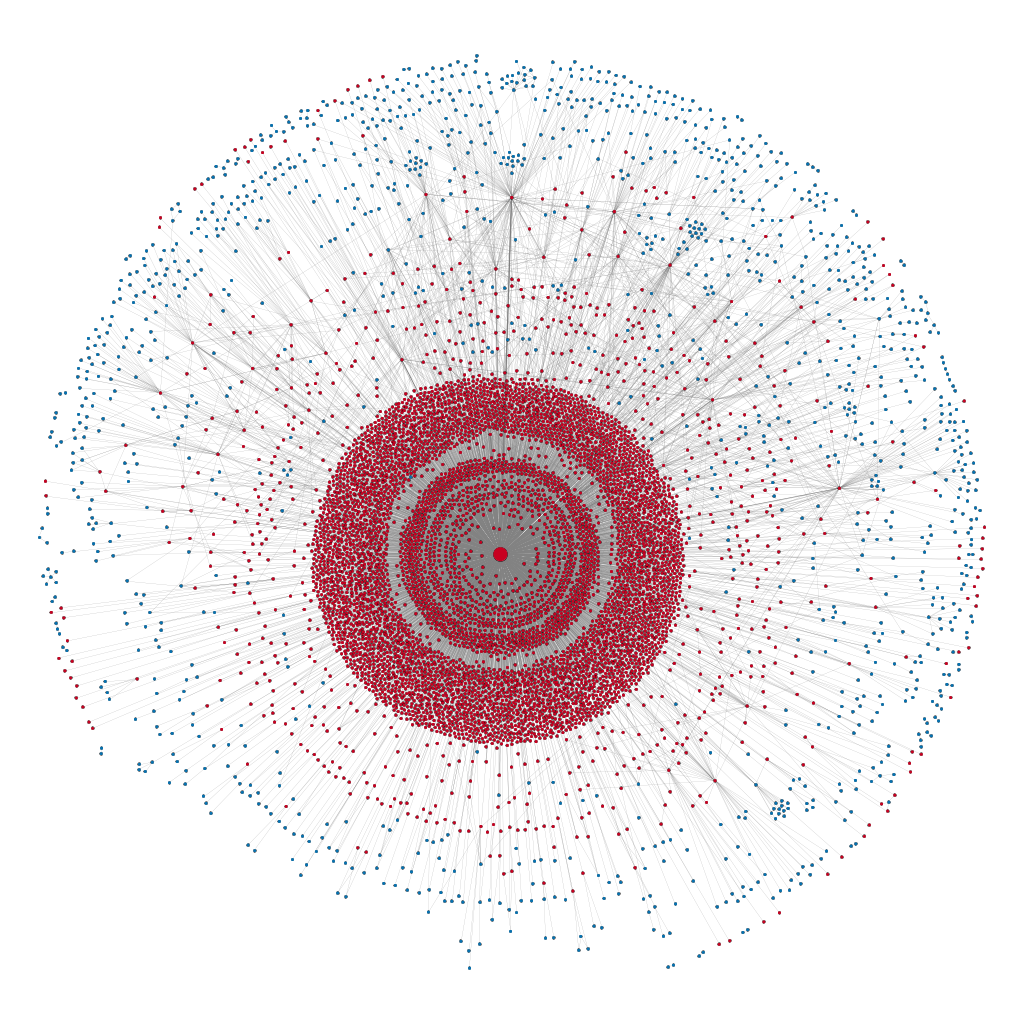
\includegraphics[scale=0.20]{prodigy_network_John_V.png}}
	\subfigure{\label{fig:evol} 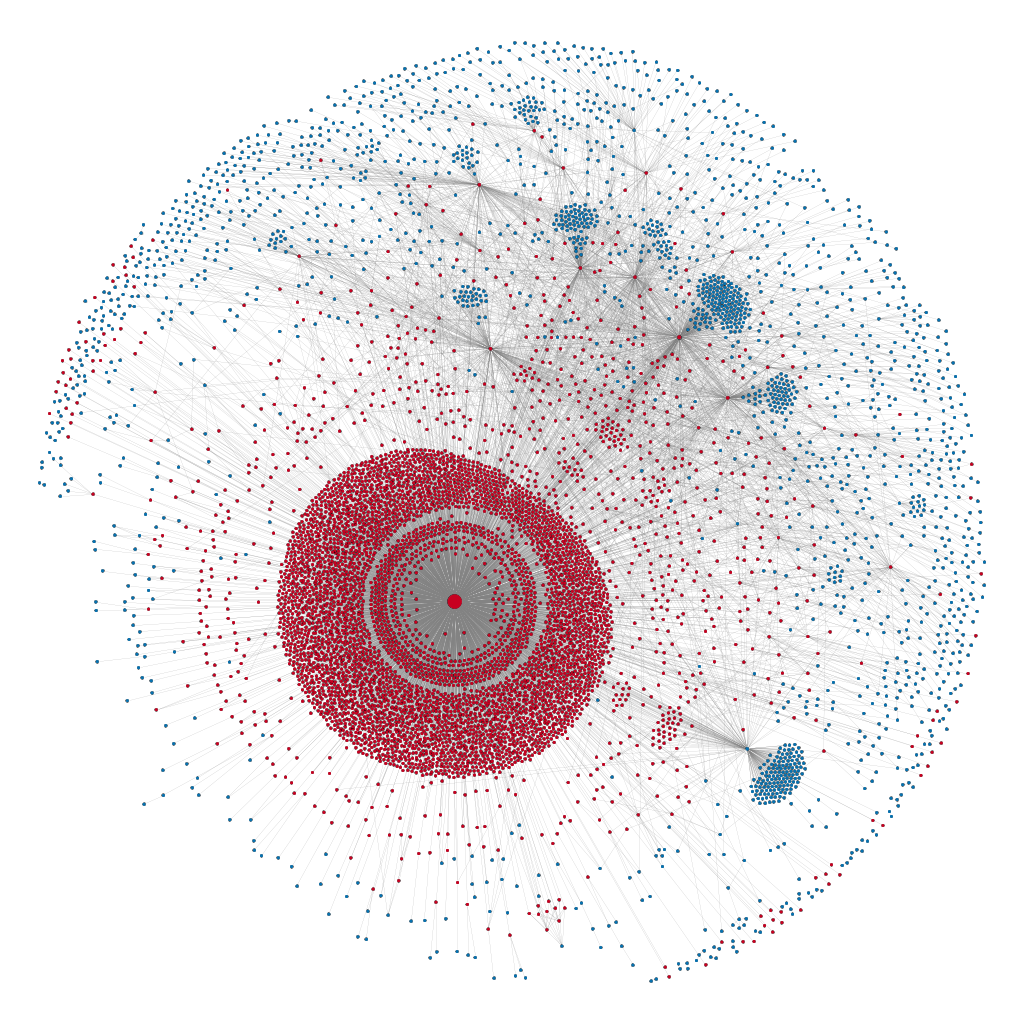
\includegraphics[scale=0.20]{prodigy_network_Joseph_I.png}}
	\put(-395,180){(A)}
	\put(-190,180){(B)}
	\caption{Communication networks during the reign of (A) John V, and (B) Joseph I. Red nodes are the monarch (in the center of the red arc) and its respective ego-network, showing that citizens of the whole empire could reach the monarch directly. Other high degree nodes correspond to government officials acting like hubs. These are mostly secretaries and governors (c.f. Tables \ref{tb:in_john} to \ref{tb:out_joseph}).}
	\label{fig:net_viz}
\end{figure*}

\begin{table}[]
	\vspace{0.2cm}
	%\small
	\centering
	\caption{Top 10 actors with the highest in-degree during the reign of John V, excluding the monarch. N/A = Not applicable, meaning that the governors, for instance, do not have an institutional affiliation.  \label{tb:in_john}}
	\vspace{0.2cm}
	\begin{tabular}{|p{4cm}|c|p{4cm}|p{4cm}|}
		\hline
		\multicolumn{1}{|c|}{Actor}              & \multicolumn{1}{l|}{In-degree} & \multicolumn{1}{c|}{Occupation}                   & \multicolumn{1}{l|}{Institutional affiliation}       \\ \hline
		Manuel Caetano Lopes de Lavre            & 64                             & Secretary                                         & Overseas Council                                     \\ \hline
		Gomes Freire de Andrade                  & 43                             & Governor and Captain General                      & N/A                                                  \\ \hline
		Diogo de Mendonça Corte Real (1658-1736) & 36                             & Secretary                                         & State                                                \\ \hline
		André Lopes de Lavre                     & 34                             & Secretary                                         & Overseas Council                                     \\ \hline
		António Guedes Pereira                   & 24                             & Secretary                                         & Secretariat of State, Navy and Conquered Territories \\ \hline
		Rodrigo César de Meneses                 & 21                             & Governor and Captain General                      & N/A                                                  \\ \hline
		Vasco Fernandes César de Meneses         & 18                             & Viceroy and Captain General                       & N/A                                                  \\ \hline
		Antônio Luís de Távora                   & 17                             & \multicolumn{1}{l|}{Governor and Captain General} & N/A                                                  \\ \hline
		João Jacques de Magalhães                & 17                             & \multicolumn{1}{l|}{Governor and Captain General} & N/A                                                  \\ \hline
		Paulo Caetano de Albuquerque             & 16                             & \multicolumn{1}{l|}{Governor and Captain General} & N/A                                                  \\ \hline
	\end{tabular}
\end{table}

\begin{table}[]
	\vspace{0.2cm}
	%\small
	\centering
	\caption{Top 10 actors with the highest out-degree during the reign of John V, excluding the monarch. \label{tb:out_john}}
	\vspace{0.2cm}
	\begin{tabular}{|p{4cm}|c|p{4cm}|p{4cm}|}
		\hline
		\multicolumn{1}{|c|}{Actor}           & \multicolumn{1}{l|}{In-degree} & \multicolumn{1}{c|}{Occupation}                   & \multicolumn{1}{l|}{Institutional affiliation}   \\ \hline
		Gomes Freire de Andrade               & 93                             & Governor and Captain General                      & N/A                                              \\ \hline
		Rodrigo César de Meneses              & 61                             & Governor and Captain General                      & N/A                                              \\ \hline
		Bartolomeu de Siqueira Cordovil       & 42                             & Provider                                          & N/A                                              \\ \hline
		Francisco Cordovil de Sequeira e Melo & 39                             & Provider                                          & Royal Department of Economy                      \\ \hline
		Diogo de Mendonça Corte Real          & 35                             & Secretary                                         & Secretariat of Navy and the Overseas Territories \\ \hline
		Sebastião Bravo Botelho               & 35                             & Judge (Ouvidor Geral) and Provider                & N/A                                              \\ \hline
		Luís Vaía Monteiro                    & 34                             & Governor and Captain General                      & N/A                                              \\ \hline
		João Jacques de Magalhães             & 30                             & \multicolumn{1}{l|}{Governor and Captain General} & N/A                                              \\ \hline
		D. Luís de Mascarenhas                & 29                             & \multicolumn{1}{l|}{Governor and Captain General} & N/A                                              \\ \hline
		Caetano de Melo e Albuquerque         & 29                             & \multicolumn{1}{l|}{Coronel}                      & Cavalry                                          \\ \hline
	\end{tabular}
\end{table}

\begin{table}[]
	\vspace{0.2cm}
	%\small
	\centering
	\caption{Top 10 actors with the highest in-degree during the reign of Joseph I, excluding the monarch. \label{tb:in_joseph}}
	\vspace{0.2cm}
	\begin{tabular}{|p{4cm}|c|p{4cm}|p{4cm}|}
		\hline
		\multicolumn{1}{|c|}{Actor}          & \multicolumn{1}{l|}{In-degree} & \multicolumn{1}{c|}{Occupation}                     & \multicolumn{1}{l|}{Institutional affiliation} \\ \hline
		Francisco Xavier de Mendonça Furtado & 443                            & Secretary                                           & Secretariat of State, Navy and Overseas        \\ \hline
		Tomé Joaquim da Costa Corte Real     & 198                            & Secretary                                           & Secretariat of State, Navy and Overseas        \\ \hline
		Martinho de Melo e Castro            & 194                            & Secretary                                           & Secretariat of State, Navy and Overseas        \\ \hline
		Sebastião José de Carvalho e Melo    & 181                            & Secretary                                           & Secretary of the Kingdom and Royal Mercy       \\ \hline
		Diogo de Mendonça Corte Real         & 154                            & Secretary                                           & Secretariat of State, Navy and Overseas        \\ \hline
		Gomes Freire de Andrade              & 69                             & Governor and General Captain                        & N/A                                            \\ \hline
		Baltasar Manuel Pereira do Lago      & 37                             & Governor and General Captain                        & N/A                                            \\ \hline
		Joaquim Miguel Lopes de Lavre        & 34                             & \multicolumn{1}{l|}{Secretary}                      & Overseas Council                               \\ \hline
		Francisco Xavier de Mendonça         & 19                             & \multicolumn{1}{l|}{Secretary}                      & Secretariat of State, Navy and Overseas        \\ \hline
		Henrique Guilhon                     & 19                             & \multicolumn{1}{l|}{Judge (Juiz de Fora), Provider} & Royal Department of Economy                    \\ \hline
	\end{tabular}
\end{table}

\begin{table}[]
	\vspace{0.2cm}
	%\small
	\centering
	\caption{Top 10 actors with the highest out-degree during the reign of Joseph I, excluding the monarch. \label{tb:out_joseph}}
	\vspace{0.2cm}
	\begin{tabular}{|p{4cm}|c|p{4cm}|p{4cm}|}
		\hline
		\multicolumn{1}{|c|}{Actor}                                                  & \multicolumn{1}{l|}{In-degree} & \multicolumn{1}{c|}{Occupation}                   & \multicolumn{1}{l|}{Institutional affiliation} \\ \hline
		Diogo de Mendonça Corte Real                                                 & 127                            & Secretary                                         & Secretariat of State, Navy and Overseas        \\ \hline
		Gomes Freire de Andrade                                                      & 113                            & Governor and Captain General                      & N/A                                            \\ \hline
		Francisco Xavier de Mendonça Furtado                                         & 83                             & Secretary                                         & Secretariat of State, Navy and Overseas        \\ \hline
		D. Luís Antônio de Sousa Botelho Mourão                                      & 54                             & Governor and Captain General                      & N/A                                            \\ \hline
		José Roberto Vidal da Gama                                                   & 53                             & Secretary                                         & Secretariat of State, Navy and Overseas        \\ \hline
		Tomé Joaquim da Costa Corte Real                                             & 43                             & Secretary                                         & Secretariat of State, Navy and Overseas        \\ \hline
		João Gomes Ferreira                                                          & 42                             & Judge (Ouvidor Geral)                             & N/A                                            \\ \hline
		D. Luís de Almeida Portugal Soares de Alarcão Eça e Melo Silva e Mascarenhas & 38                             & \multicolumn{1}{l|}{Viceroy of Brazil}            & N/A                                            \\ \hline
		Francisco Cordovil de Sequeira e Melo                                        & 38                             & \multicolumn{1}{l|}{Providor}                     & Royal Department of Economy                    \\ \hline
		José António Freire de Andrade                                               & 37                             & \multicolumn{1}{l|}{Governor and Captain General} & N/A                                            \\ \hline
	\end{tabular}
\end{table}

The purpose of showing the networks and descriptives in this section is primarily to give a taste of the data and available information. More detailed and substantively-oriented analyzes are subject of our current research. We are signaling types of research questions that are on our agenda in the following Discussion.

\section{Discussion}

Our primary motivation for writing this article was to demonstrate how massive unstructured archival information is used to build network data interesting to historians and (social) network scientists. We close the article with two sets of conclusions. Firstly, technical ones related to our experiences of processing unstructured material into structured data amenable for social network analysis. Secondly, more substantive ones related to the advantages and disadvantages of the presented dataset for the historical research on early-modern Portuguese Empire.

On the technical side, constructing a dataset from textual information is not an easy task even if human effort is augmented with machine learning algorithms and fast computers. If we assume that manual coding a single document from our corpus would take 15 minutes then a single person working 8 hours a day 7 days a week would spend about 14 years coding the entire corpus. A computer trained on a small subset of human-coded documents can do that in a matter of minutes. Albeit perhaps not as accurately. One of the greatest concerns of historians regarding the use of complex automatic document processing mechanisms to perform the historical analysis is the risk of simplifying registered information, which may affect the reliability of the final research results. Therefore, we decided to use Regular Expressions, thanks to which we checked whether the sequences matched our specific patterns, and then, by using Named Entity Recognition, we managed to classify entities into predefined categories. It is worth noting that when preparing historical documents for further data analysis, we shall always check manually some of the stored data in such a way that the training model can learn from data and perform in more accurate way. The more accurate the training data, the more accurate the final text classification results.

We formulate the following recommendations regarding the data challenges in extracting data from historical texts from a broader perspective.  Before analyzing the text and preparing the appropriate algorithms, one should consider which words actually need such algorithms and which ones are identifiable via more straightforward keyword search. In our dataset we needed algorithms primarily to identify people (due to the specificity of Portuguese names) but also to identify and classify institutions according to their political, religious, or military character, because the vocabulary changed over time due to the administrative development of the Portuguese empire. Issues related to religious and ethnic minorities do not require separate algorithms and can be easily identified through keywords.

Regarding text structure, we consider Regular Expressions an extremely helpful tool for finding patterns in the text and to identify the pieces of text containing key information. We have learned that even unstructured documents can have patterns, so it might make all the difference spending some time trying to find them. In historical network analysis we need to deal with an extremely large number of unstructured text at once and it can make the data analysis ever more complicated. Therefore, we recommend the researchers to split the study into several smaller data sets to be addressed one at a time. A small data set can be manually checked and then used as input to the machine learning models, which are in turn used on the next set of documents to be studied. We believe this can reduce the total amount of manual work and improve the quality of the models. As far as manual work is concerned, it is crucial to be guided by quality not quantity. The long hours of manual work on coding and checking the accuracy of the algorithms is by far the most “expensive” resource of a researcher. Low quality output will most likely lead to repeating other manual tasks.

The methods we describe in this article should be helpful for documents that are official correspondence. The algorithms we mentioned helped us to determine information about senders and recipients as well as their social attributes and geographic locations. However, the historians are working on various sources from different historical eras and various archives. We believe that the methodology we have described may help in setting the first steps to convert other types of historical documents into network data.

On the substantive side, the corpus consists primarily of letters and other documents that can be interpreted as official but interpersonal communication: senders and recipients are persons not collectives or institutions. Still, the data should not be treated as a complete communication network. Letters and documents usually stay by the recipient and our corpus comes from an archive in Lisbon. As a result the majority of the documents in the corpus are sent to the officials residing in Lisbon and we are lacking the replies and other documents sent from the officials residing in Lisbon to, say, governors of overseas colonies. Nevertheless, the data provides a broader perspective of what types of social and political actors, with underprivileged groups in particular, communicated with the King and Empire's capital.

We believe the dataset we are constructing has a much larger research potential than we were able to present in this article. Among the immediate ones are for example whether the appearance of high degree actors during the reigns of subsequent monarchs (as shown in Figures \ref{fig:degree_dist} and \ref{fig:net_viz}) is an evidence of changes in governance towards the monarch delegating some tasks to his subordinate officials. Are there differences between networks in different colonies? Do different governmental positions correspond to structurally equivalent network positions? How does the inter-institutional network look like and how does it change over time? Further enrichment of the constructed dataset enabling addressing other interesting historical research questions is on our agenda. We mention two of them here. Firstly, the data provides not only the information about who sends a document to whom, but also about what. We plan to use methods of ``topic modeling'', such as Latent Dirichlet Allocation \cite{blei_latent_2003}, to cluster the documents to groups according to their content. It might be possible to identify main topics and their changing popularity throughout the whole period and across geographical locations. Secondly, the authors write the documents mentioning other people, events and places. We are investigating methods through which our corpus can be used as a source of such “indirect” information about events, persons, geographical locations and social relations between them. Similar goals were pursued by \cite{warren_six_2016} in their analysis of the Oxford Dictionary of National Biography. In other words, to construct a network data that also involves people who were not senders or recipients, but were mentioned by others in their communications.


\section*{Acknowledgments}
Research presented in this article is a part of The Portuguese Overseas Identity project. Authors are very grateful to two anonymous reviewers for the work they invested in giving constructive comments that helped to significantly improve the article.  Agata Błoch thanks (Polish) National Science Centre (grant 2017/27/N/HS3/01104), and Tadeusz Manteuffel Institute of History of Polish Academy of Sciences for support. Authors also thank Jessica Joia, Bartosz Lemiec, and Monika Pawluczuk for their contributions to data preparation and processing. We are also  grateful to Lina Oliveira Lopes-De Matos and his students from University Marie Curie-Sklodowska in Lublin for their help in annotating the source documents. 


\bibliographystyle{unsrt}  
\bibliography{networks_from_archives}

\end{document}
